%version of 08-23-18

\chapter{SUMMATION}
\label{ch:Summation}


\section{Introduction}
\label{sec:intro}

The operation of {\it summation}---adding up aggregates of
numbers---is of fundamental importance in the world of digital
computing.  While we humans are able to deal handily with abstractions
such as ``smoothness'' and ``continuity'', we must employ
sophisticated {\em discretizations} of these concepts in order to
enlist the aid of digital computers in dealing with such abstractions.
Summations provide a very useful discretization of ``continuous'' or
``smooth'' phenomena that are typically dealt with by humans with the
aid of the (differential and integral) calculus that was invented by
Newton and Leibniz for such dealings.

This chapter is dedicated to exploring how to employ summations as a
computational tool.  We deal throughout with {\it series}, {\it i.e.},
(possibly infinite) sequences of numbers
\[ a_1, a_2, \ldots \]
whose sum
\begin{equation}
\label{eq:abstract-sum}
a_1 + a_2 + \cdots
\end{equation}
is of interest.
\begin{quote}
{\em Of course, when we deal with {\em infinite} series, wherein there
  are infinitely many numbers $a_i$, we must address the question of
  whether the sum (\ref{eq:abstract-sum}) exists as a finite number.
  For some infinite series the sum {\em does} exist as a finite
  number, as with the well-known sum
\begin{equation}
\label{eq:sample-sum-2^(-k)}
 1 \ + \ \frac{1}{2} \ + \ \frac{1}{4} \ + \ \frac{1}{8} \ +
\ \frac{1}{16} \ + \ \cdots \ + \ \frac{1}{2^k}  \ +
\ \frac{1}{2^{k+1}} \ + \ \cdots \ = \ 2 
\end{equation}
%{\Denis Here we can refer to the Achille and Tortoise story as this corresponds to the distance Achille's did to reach the tortoise if the initial situation is 1 meter...}
Such an infinite series is said to {\em converge}.
\index{infinite series!convergent}

But sometimes an infinite series {\em does not} have a finite
  sum.  This is true, for instance, with the well-known {\it harmonic}
  series \index{harmonic series}
\begin{equation}
\label{eq:sample-sum-harmonic}
1 \ + \ \frac{1}{2} \ + \ \frac{1}{3} \ + \ \frac{1}{4} \ +
\ \frac{1}{5} \ + \ \cdots \ + \ \frac{1}{k} \ + \ \frac{1}{k+1} \ +
\ \cdots
\end{equation}
As more and more terms are added, the accumulated sum eventually
exceeds every number.  Such an infinite series is said to {\em diverge}.
\index{infinite series!divergent}

%{\Denis There is a link between harmonic series and the frequencies
%of the notes in music (each note corresponds to the fundamental
%divided by 2, 3, 4, ... May be it would be nice here to develop?}
%{\Arny I do not know enough to say anything intelligent about this.}
}
\end{quote}

\begin{quote}
{\em Sums such as (\ref{eq:sample-sum-2^(-k)}) and
  (\ref{eq:sample-sum-harmonic}) illustrate some of the complexity of
  dealing with infinite entities.  Most obviously, as we have just
  remarked, when the sums are infinite, some of them have finite sums
  while others do not.  Even more subtle, the series that {\em do}
  have (finite) sums illustrate the unintuitive fact that, sometimes
  finite objects or entities---such as the integer $2$ in
  (\ref{eq:sample-sum-2^(-k)})---have infinite ``names''---the
  infinite series in this example.  Lots to think about!
}
\end{quote}

\begin{quote}
{\em
The complexity of the concept of convergence has been recognized in
various forms for more than $25$ centuries.  Several charming and
familiar examples appear in the paradoxes attributed to Zeno of Elea.
In his {\it Paradox of Achilles and the Tortoise}, for instance, Zeno
appears to prove that all motion is illusory.  In this story, the
slow-footed Tortoise (T) tries to convince the speedy Achilles (A) of
the futility of trying to win any race in which A gives T even the
smallest head start.  As long as T is ahead of A, says T, every time A
traverses half the distance between the competitors, T will respond by
moving a bit further ahead.  Thereby, T will always be a positive
distance ahead of A, so that A can catch T.  A similar ``argument''
demonstrates that an arrow shot at you by an adversary can never reach
you, as long as you continually move away from the archer.  {\em DO
  NOT TRY THIS AT HOME!!}

The subtleties of the notion of {\em infinitesimals} that explains the
fallacy of assertions such as the Tortoise's was not well understood
until a few hundred years ago.

The general topic of the convergence or divergence of infinite series
is beyond the scope of this text.  It is a fascinating subject for
advanced study.
}
\end{quote}


Toward the end of guiding the reader through the forest of
abstractions and operations and techniques associated with summations,
we categorize the targets of our discussions in three ways.
\begin{enumerate}
\item
We study a number of {\it fundamental sums} that have intrinsic
interest.
%{\Denis Notice here that none of the following examples are arithmetic or geometric...}
Examples of this topic category include {\it arithmetic summations},
{\it geometric summations}, and {\it mathematically ``smooth''
  summations}, including sums of positive and negative powers of
integers.  Here is a sampler of summations that appear in this
chapter.
\[
\begin{array}{lcl}
1 \ + \ 2 \ + \ 3 \ + \ 4 \ + \ 5 \ + & \cdots & + \ k  \ + \ (k+1) \ +
\ \cdots \ + \ n \\
1 \ + \ 2 \ + \ 4 \ + \ 8 \ + \ 16 \ + & \cdots & + \ 2^k  \ +
\ 2^{k+1} \ + \ \cdots \ + \ 2^n \\
1 \ + \ 4 \ + \ 9 \ + \ 16 \ + \ 25 \ + & \cdots & + \ k^2  \ + \ (k+1)^2 \ +
\ \cdots \ + \ n^2 \\
1 \ + \ \frac{1}{2} \ + \ \frac{1}{4} \ + \ \frac{1}{16} \ +
\ \frac{1}{32} \ + & \cdots & + \ \frac{1}{2^k}  \ + \ \frac{1}{2^{k+1}} \ +
\ \cdots \\
1 \ + \ \frac{1}{2} \ + \ \frac{1}{3} \ + \ \frac{1}{4} \ +
\ \frac{1}{5} \ + & \cdots & + \ \frac{1}{k}  \ + \ \frac{1}{k+1} \ +
\ \cdots \\
1 \ + \ \frac{1}{4} \ + \ \frac{1}{9} \ + \ \frac{1}{16} \ +
\ \frac{1}{25} \ + & \cdots & + \ \frac{1}{k^2}  \ + \ \frac{1}{(k+1)^2} \ +
\ \cdots
\end{array}
\]

\item
We study a variety of {\it fundamental techniques} for performing
summations.

We include specialized techniques that work for specific classes of
summations, as well as more general techniques that work in a broad
range of situations.

Examples of such techniques include, e.g.: estimating summations by
integrating functions related to the summation; grouping/replication
of terms within a summation; verifying ``guessed'' sums via induction.

\item
We study a variety of {\it fundamental representations} of the
elements being summed.  We observe that being able to study the same
phenomenon in a variety of seemingly unrelated ways often gives one
unexpected mathematical understanding of and operational control over
the phenomenon.

Examples of such representations include, among others,
representations of numbers by: numerals in a positional number system;
slices of pie; tokens arranged in stylized ways; basic geometrical
structures, including the unit-width rectangles of Riemann sums.
\end{enumerate}

\medskip

\noindent
{\em In summation, we treat each topic in multiple ways, as long as
  each new way teaches a new lesson.}

\bigskip

%%%%%%%%%%%%%%%%%%%%%%%%%%%%%%%%%%%%%%%%%%%%%%%%





\ignore{\Denis Again, as I said before, I am not really convinced by this example.
Keeping the same sum, I prefer the story of Sissa, telling an old legende:
where wheat or rice is placed upon each square of the chess board in the following way:
put one grain on the first square, and then, double this number on each of the subsequent squares,
$2$ in the second case, $4$ in the third and so on.}

\ignore{\Denis add cross reference for computing the sum of powers of 2 in DOINGMATHS}

To illustrate the power of summation methodology, consider the
following modernized version of the {\it legend of Sissa ibn Dahir}
\index{Sissa ibn Dahir, legend of} who has invented a marvelous game,
let's call it {\it chess}, that is played on an $8 \times 8$ array of
unit-size squares---call it a {\it chessboard}.  A benefactor offers
you a one-time gift of {\em one million million (i.e., $10^{12} =
  1,000,000,000,000$) euros} in return for all rights to the game.  As
a counter-offer, you ask your benefactor instead for all of the money
amassed in the following way.  You ask your benefactor to proceed row
by row along a chessboard, placing money in the board's squares,
according to the following regimen.  Your benefactor should place $1$
euro in the first square, $2$ euros in the second square, $4 \ (= 2
\times 2)$ euros in the third, $8 \ (= 4 \times 2)$ euros in the
fourth, and so on, doubling the number of euros at each step of the
procedure---so the last square would contain $2^{63}$ euros.
Fig.~\ref{fig:Sissa} provides an illustration of the growing of the first steps of the filling process.
\noindent
{\em Have you made a good bargain?}
\begin{figure}[ht]
\begin{center}
       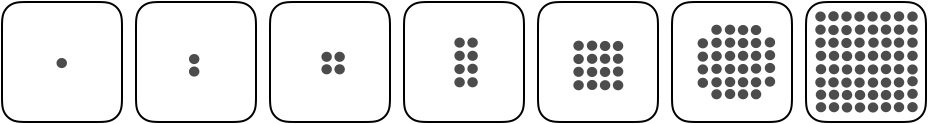
\includegraphics[scale=0.3]{FiguresMaths/chess}
\caption{First filled board's squares.}
       \label{fig:Sissa}
\end{center}
\end{figure}

By the end of this chapter, you will be able to determine in minutes
that under your procedure (the one that uses the chessboard), you
would receive $2^{64} -1$ euros---which is more than $10^{20}$ euros,
hence {\em much} more than the mere $10^{12}$ euros that your
``benefactor'' offered you!
%{\Denis I think the previous value is -1 and not -2}

\noindent
{\em A good bargain, indeed!}

%%%%%%%%%%%%%%%%%%%%%%%%%%%%%%%%%%%%%%%%%%%%%%%%%%%%


\section{Summing Structured Series}
\label{sec:structured-series}

\subsection{Arithmetic Sums and Series}
\label{sec:arithmetic-series}

\subsubsection{General development}

We define arithmetic sequences and learn how to calculate their sums.

\begin{equation}
\label{eq:arith-seq}
\begin{array}{l}
\mbox{An $n$-term arithmetic sequence:} \\
\hspace*{.25in}a, \ a+b, \ a+2b, \ a+3b, \ \ldots, a+(n-1)b \\
\\
\mbox{The corresponding arithmetic series:} \\
\hspace*{.25in}a + (a+b) + (a+2b) + (a+3b) + \cdots + (a+(n-1)b) \\
\hspace*{.5in} = \
an + b \cdot (1 + 2 + \cdots + n-1)
\end{array}
\end{equation}
We can, thus, sum the arithmetic series in (\ref{eq:arith-seq}) by
determining the sum of the first $m$ positive integers; $m = n-1$ in
(\ref{eq:arith-seq}).  We use this result as an opportunity to
introduce important notation.

\subsubsection{Special cases}

\paragraph{\sf A. Summing the first $n$ integers: the case $a=b=1$}
Our first goal is to sum the first $n$ positive integers:
\[ 1 \ + \ 2 \ + \cdots + \ n , \]
that is, to find a {\it closed-form expression} 
\index{closed-form expression}
for the sum.  In somewhat informal terms, we say that an expression of
the form
\[ f(n) \ \eqdef \ \sum_{i=1}^n \ i \]
is in {\it closed form} if it exposes a prescription for evaluating
the sum using a {\em fixed-length} sequence of arithmetic operations
(e.g., addition/subtraction, multiplication/division,
exponentiation/taking logarithms).

The desired sum $f(n)$ is commonly denoted $\Delta_n$.
\index{$\Delta_n$: sum of the first $n$ integers}
We usually prefer the notation $S_1(n)$ for this sum because it
exposes this summation as an instance of a related family of such
summations that will occupy us through this chapter.

The remainder of subsection A is devoted to developing multiple ways
to derive the following (closed-form) expression for $\Delta_n =
S_1(n)$.

\begin{prop}
\label{thm:sum-first-integers-Gauss}
\index{sum of first $n$ integers}
For all $n \in \N$,
\begin{equation}
\label{eq:sum-1-to-n}
S_1(n) \ = \ \sum_{i=1}^n \ i \
  \ = \  \frac{1}{2} n (n+1) 
\end{equation}
\end{prop}
\index{Sum of the first $n$ integers: $\Delta_n = S_1(n)$}

%{\Denis I removed the last equality with n+1 choose 2 since this
%combinatorial proof is presented later...}

\index{Sum of the first $n$ integers: $\Delta_n = S_1(n)$!a {\bf
    textual} derivation}
\begin{proof}
{\bf A textual proof.}
\index{sum of first $n$ integers!a textual reckoning}
%
We begin with a {\em constructive} proof\footnote{The proof is {\em
    constructive} in that it actually derives an answer.  This is in
  contrast to, say, the inductive validation of the sum in
  Section~\ref{sec:positive-integer-power}.C, which just verifies a
  ``guessed'' answer.}~of summation (\ref{eq:sum-1-to-n}) that employs
an approach known to the eminent German mathematician Karl Friedrich
Gauss \index{Gauss, Karl Friedrich} as a pre-teenager.  \index{Gauss,
  Karl Friedrich!summation ``trick''} This approach proceeds in two
steps.
\begin{equation}
\label{eq:arith-series}
\begin{array}{llccccccccc}
\mbox{Write $S_1(n)$ ``forwards'':} &
\hspace*{.2in}\sum_{i=1}^n \ i \ = & 1 & + & 2   & + & \cdots & + & (n-1) & + & n \\
 & & & & & & & & & &  \\
\mbox{Write $S_1(n)$ ``in reverse'':} &
\hspace*{.2in}\sum_{i=n}^1 \ i \ = & n & + & (n-1) & + & \cdots & + & 2   & + & 1
\end{array}
\end{equation}
Now add the two representations of $S_1(n)$ in (\ref{eq:arith-series})
{\em columnwise}.  Because each of the $n$ column-sums equals $n+1$,
we find that $2 S_1(n) = n(n+1)$, which we easily rewrite in the form
(\ref{eq:sum-1-to-n}) (after multiplying both sides of the equation by
$2$).
\end{proof}

\medskip

\noindent {\bf Remark.}
%
{\em Now is an opportune moment to step back from the specific result
  in Proposition~\ref{thm:sum-first-integers-Gauss} and concentrate on
  the textual proof.  What Gauss noticed about the sum of the first
  $n$ integers is that when the sum is doubly written as in
  (\ref{eq:arith-series}), the column-sums are all the same.  This
  phenomenon of {\em finding invariants} is a ``pattern'' of the form
  referred to in Section~\ref{sec:manifesto} as we discussed how
  mathematicians ``do mathematics''.  We see in the proof how the
  pattern can be exploited to determine sum of any arithmetic series.
  {\em What seemed to be a ``trick'' turns out to be an insightful
    instance of pattern-matching.}  We shall soon see that the pattern
  can be exploited to other, related, ends.}

\medskip

Not everyone thinks the same way---even within the context of
mathematics.  It is, therefore, very important for the reader to
recognize that even the simplest mathematical facts can be proved and
analyzed in a broad variety of ways.  We illustrate this assertion by
developing more proofs of
Proposition~\ref{thm:sum-first-integers-Gauss}.

\index{Sum of the first $n$ integers: $\Delta_n = S_1(n)$!a {\bf
    ``pictorial'', graphic} derivation}
\begin{proof}
{\bf A ``pictorial'', graphic proof.}
%
The idea now is to look at the problem of summing the first $n$
integers as a problem of estimating the area of a simple (in the
\textit{good sense} of the word) surface.  In this worldview, integers
are represented by concatenating basic {\it unit-side} (i.e., $1
\times 1$ \index{unit-side square} {\it squares}), as in
Fig.~\ref{fig:sumIntegersGeo1}.

Our summation process can be obtained in three steps, in the manner
illustrated by the three figures
Figs.~\ref{fig:sumIntegersGeo1},~\ref{fig:sumIntegersGeo2},
and~\ref{fig:sumIntegersGeo3}.
\begin{figure}[ht]
\begin{center}
       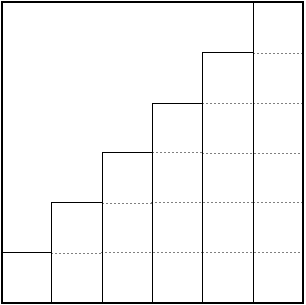
\includegraphics[scale=0.4]{FiguresMaths/SumIntegersGeometricBasis}
\caption{Representing the first $n$ integers using basic unit squares; $n=6$ in this example.}
       \label{fig:sumIntegersGeo1}
\end{center}
\end{figure}
\begin{figure}[ht]
\begin{center}
       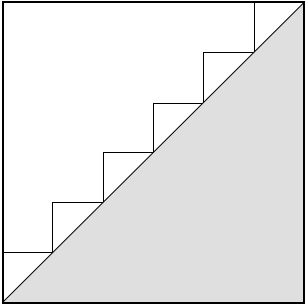
\includegraphics[scale=0.4]{FiguresMaths/SumIntegersGeometricIntermediate}
\caption{The area of the lower-right triangle (light grey) is one-half that of
  the entire $n \times n$ square.}
       \label{fig:sumIntegersGeo2}
\end{center}
\end{figure}
\begin{figure}[ht]
\begin{center}
       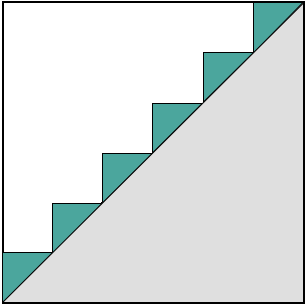
\includegraphics[scale=0.4]{FiguresMaths/SumIntegersGeometricFinal}
\caption{The area of the (dark) triangles sitting on the upper
  diagonal of the $n \times n$ square is $\frac{1}{2} n$.}
       \label{fig:sumIntegersGeo3}
\end{center}
\end{figure}
\begin{enumerate}
\item
We begin, in Fig.~\ref{fig:sumIntegersGeo1}, by depicting the problem
calculating $S_1(n)$ as the problem of determining the area of a
surface constructed from unit-side squares.

\item
Next, we illustrate in Fig.~\ref{fig:sumIntegersGeo2} that the area of
the lower-right triangle of the $n \times n$ square---depicted in
light grey in the figure---is one-half that of the entire $n \times n$
square.

\item
Finally, we indicate in Fig.~\ref{fig:sumIntegersGeo3} that the area
of the small (dark grey in the figure) triangles that cover the upper
diagonal of the $n \times n$ square is $\frac{1}{2} n$.  This
reckoning notes that there are $n$ triangles, and each has an area
that is one-half that of a unit-side square.
\end{enumerate}
We thereby reckon the area of the surface depicting $S_1(n)$ as

\begin{tabular}{l}
{\it One-half the area of the $n \times n$ square,
i.e., $\frac{1}{2} n^2$} \\
\hspace*{.15in} plus   \\
{\it $n$ times the area of one-half a unit-side square,
i.e., $\frac{1}{2} n$}
\end{tabular}

\noindent
We have, thus, derived the value of $S_1(n)$.
\end{proof}

\medskip

We present one final proof of
Proposition~\ref{thm:sum-first-integers-Gauss}.

\index{Sum of the first $n$ integers: $\Delta_n = S_1(n)$!a {\bf
    combinatorial} derivation}
\begin{proof}
{\bf A combinatorial proof.}
%
The following argument is {\it combinatorial} in that it achieves its
goal by {\em counting} instances of the first $n$ integers, laid out
in a line.

Place (tokens that represent) the integers $0$ to $n$ along a line.
For each integer $i$, count how many integers $j > i$ lie to its
right.  We see that in general, there is a {\it block} of $n-i$
integers that lie to the right of integer $i$.  In detail: the block
of integers lying to the right of $i=0$ contains $n$ values of $j$;
the block to the right of $i=1$ contains $n-1$ values of $j$, and so
on, as suggested in Fig.~\ref{fig:rightward-instances}.

\begin{figure}[htb]
\[
\begin{array}{lcccccc}
\mbox{All integers $\leq 4$:} &
 & 0 & 1 & 2 & 3 & 4 \\
\mbox{integers to the right of $0$:} &
 &   & 1 & 2 & 3 & 4 \\
\mbox{integers to the right of $1$:} &
 &   &   & 2 & 3 & 4 \\
\mbox{integers to the right of $2$:} &
 &   &   &   & 3 & 4 \\
\mbox{integers to the right of $3$:} &
 &   &   &   &   & 4
\end{array}
\]
\caption{A two-dimensional depiction of the right-lying
  integer-instances.}
\label{fig:rightward-instances}
\end{figure}

On the one hand, we see that the total number of right-lying integers
$j$ equals $n+(n-1)+ ... + 1 \ = \ S_1(n)$.

On the other hand, every instance of a right-lying integer can be
identified uniquely by the pair of nonnegative integers, $i$ (the
instance's block) and $j>i$ (the instance's position-within-block).
The total number of right-lying integer-instances corresponds to the
number of ways to select two integers from among $n+1$.\footnote{We
  study such counting techniques in depth in
  Section~\ref{sec:counting}.}  This number is the binomial
coefficient whose definition we specialize from
(\ref{eq:binom-coeff}) Section~\ref{sec:binary-operators}.C:
\index{binomial coefficient}
\[ 
\Delta_n \ = \ {{n+1} \choose 2} \ \eqdef \ \frac{1}{2} n(n+1).
\]

We have thus derived two distinct---but, of course,
equal---expressions for $S_1(n)$.
\end{proof}

\begin{quote}
{\em Our combinatorial derivation of the sum (\ref{eq:sum-1-to-n})
  illustrates one of the most important roles of mathematical
  abstraction.  There is no obvious intuition to explain the
  relationship between the activity of summing $n$ consecutive
  integers and the activity of extracting two items out of a set of
  $n$ items.  Yet, our combinatorial derivation exposes an intimate
  connection between the two. }
\end{quote}

\medskip

Now that we know---{\em and understand}---how to derive the value of
$S_1(n)$, we can finally evaluate our original series in
(\ref{eq:arith-seq}).  \index{arithmetic series:explicit sum}

\begin{prop}
\label{thm:sum-of-arithmetic-series}
The arithmetic series in (\ref{eq:arith-seq}) has the sum
\begin{equation}
\label{eq:sum-arithmetic-series}
a + (a+b) + (a+2b) + (a+3b) + \cdots + (a+(n-1)b) \ \ = \ \
%an + b \cdot {n \choose 2}. 
an + b \cdot \Delta_n. 
\end{equation}
\end{prop}


\paragraph{\sf B. Perfect squares are sums of odd integers}
In this section, we build on
Proposition~\ref{thm:sum-first-integers-Gauss} to craft multiple
constructive proofs of the fact that each perfect square, say, $n^2$,
is the sum of the first $n$ odd integers, $1, 3, 5, \ldots, 2n-1$.
All of these proofs complement the ``guess-and-verify'' inductive
proof of this result in Section~\ref{sec:positive-integer-power}.C.

\begin{prop}
\label{thm:squares-odd-integers-Gauss}
\index{$n^2$ as sum of first $n$ odd integers}
For all $n \in \N^+$,
\begin{equation}
\label{eq:sum-of-odds}
\sum_{k=1}^n \ (2k-1)
 \ = \ 1 + 3 + 5 + \cdots + (2n-1) \ = \ n^2.
\end{equation}
That, is, the $n$th perfect square is the sum of the first $n$ odd
integers.
\end{prop}

Before we present several proofs of this result, we note that the
notation for odd integers in (\ref{eq:sum-of-odds}) is perfectly
general: every positive odd integer $n$ can be written in the form
$2k-1$ for some positive integer $k$. 

\medskip

Our first two proofs of
Proposition~\ref{thm:squares-odd-integers-Gauss} note that the result
is a corollary of both Proposition~\ref{thm:sum-first-integers-Gauss}
and Proposition~\ref{thm:sum-of-arithmetic-series}.

The first of these proofs builds on the stratagem of {\em finding
  invariants} that we exploited in the textual proof of
Proposition~\ref{thm:sum-first-integers-Gauss}.

\medskip

\index{$n^2$ as sum of first $n$ odd integers!a proof using algebra}
\begin{proof}
{\bf A proof using algebra.}
%
By direct calculation, we find that
\begin{eqnarray*}
\sum_{k=1}^n \ \left( 2k-1 \right)
   & = & 2 \sum_{k=1}^n \ k \ \ - \ n \\
   & = & 2 \Delta_n \ \ - \ n \ \ \ \ \ \ \ \ \ \ \mbox{ (by
  Proposition~\ref{thm:sum-first-integers-Gauss})} \\
   & = & (n^2 + n) - n \\
   & = & n^2.
\end{eqnarray*}
\end{proof}

\medskip

\index{$n^2$ as sum of first $n$ odd integers!a proof by calculation}
\begin{proof}
{\bf A proof by calculation.}
%
Because summation (\ref{eq:sum-of-odds}) is an arithmetic series with
$a=1$ and $b=2$, we know from
Proposition~\ref{thm:sum-of-arithmetic-series} that the summation
evaluates to
\[ (1 \cdot n) + 2 \Delta_{n-1} \ = \ n + n^2 -n \ = \ n^2. \]
\end{proof}

\ignore{***\Denis According to the
  expression of Proposition~\ref{thm:sum-of-arithmetic-series}, the
  sum is equal to $1.n + 2 \Delta_{n-1} = n + n^2 -n = n^2$.  Let us
  detail several alternative proofs.***}

\medskip

\index{$n^2$ as sum of first $n$ odd integers!a textual proof}
\begin{proof}
{\bf A textual proof.}
%
We adapt Gauss's ``trick'', wherein one adds the series written
forwards to the series written backwards, to this summation.  Let us
denote the target sum $\sum_{k=1}^n \ (2k-1)$ by $S(n)$.  We record
$S(n)$ in two ways:
\begin{equation}
\label{eq:add-odds}
\begin{array}{llccccccccc}
\mbox{``Forwards'':} &
S(n) \ = 
& 1 & + & 3 & + & \cdots & + & (2n-3) & + & (2n-1) \\
 & & & & & & & & & &  \\
\mbox{``Backwards'':} &
S(n) \ =
& (2n-1) & + & (2n-3) & + & \cdots & + & 3 & + & 1
\end{array}
\end{equation}
Now add these two representations of $S(n)$ {\em columnwise}.  Because
each of the $n$ column-sums equals $2n$, we find that
\begin{equation}
\label{eq:sum-of-odds-sum}
2 S(n) \ = \ 2 \sum_{k=1}^n \ (2k-1) \ = \ 2n^2.
\end{equation}
We thus derive the sum (\ref{eq:sum-of-odds}) when we halve the three
equated quantities in equation (\ref{eq:sum-of-odds-sum}), i.e.,
divide each quantity by $2$.
\end{proof}

\medskip

\index{$n^2$ as sum of first $n$ odd integers!a proof ``by pictures''}
\begin{proof}
{\bf A proof ``by pictures''.}
%
We now build up to a proof that is almost purely pictorial, with just
a bit of reasoning mixed in.  The only ``sophisticated'' knowledge
required is that
\begin{equation}
\label{eq:(n+1)^2}
(n+1)^2 \ = \ n^2 \ + \ 2n \ + \ 1.
\end{equation}
\begin{quote}
{\em We remark that equation (\ref{eq:(n+1)^2}) is the simplest
  instance of the {\em restricted Binomial Theorem}, which appears
  later in this chapter as Theorem~\ref{thm:restricted-binomial-thm}.}
\end{quote}
The well-known equation (\ref{eq:(n+1)^2}) can be verified by
explicitly symbolically squaring $n+1$:
\[ (n+1) \cdot (n+1) \ \ = \ \ n \cdot (n+1) \ + \ (n+1) 
     \ \ = \ \ n^2 \ + \ n \ + \ n \ + \ 1.
\]
The equation can also be verified using the highly perspicuous
Fig.~\ref{fig:proofa2plusb2}.
%{\Denis We can remark here that this result is straightforward as
%follows. see below if you think it should be included.}
\begin{figure}[ht]
\begin{center}
       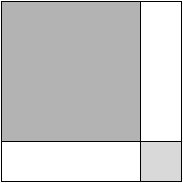
\includegraphics[scale=0.4]{FiguresMaths/proofa2plusb2}
\caption{A geometrical proof of the identity $(n+1)^2 = n^2 + 2n + 1$.}
       \label{fig:proofa2plusb2}
\end{center}
\end{figure}
The figure tells its tale by exhibiting four rectangles that make up
an $(n+1) \times (n+1)$ square; the area of this square is, of course,
$(n+1)^2$.  This large square is made up of four rectangles.
\begin{itemize}
\item
Reading across the top of the figure, we encounter a darkly shaded $n
\times n$ square (area $= n^2$) and an unshaded $n \times 1$ rectangle
(area $= n$).
\item
Reading across the bottom of the figure, we encounter an unshaded $1
\times n$ rectangle (area $= n$) and a lightly shaded $1 \times 1$
square (area = $1$).
\end{itemize}
The overall message is that $(n+1)^2$ (the area of the large,
composite, square)

\begin{tabular}{ll}
is the sum of & \\
  & $n^2$ (the area of the darkly shaded square) \\
plus & \\
  & $2n$ (the combined areas of the unshaded rectangles) \\
plus & \\
  & $1$ (the area of the lightly shaded square)
\end{tabular}

\medskip

\noindent
Back to our proof of Proposition~\ref{thm:squares-odd-integers-Gauss}.
%
Our pictorial proof begins by representing each integer $n$ as a
horizontal sequence of $n$ ``bullets'', i.e., darkened circles.  The
problem of summing the first $n$ odd integers then begins with a
picture such as appears in Fig.~\ref{fig:sumOdds1}, for the
illustrative case $n=5$.

\begin{figure}[ht]
\begin{center}
       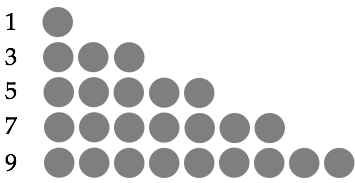
\includegraphics[scale=0.4]{FiguresMaths/SumOddsBasis}
\caption{Representing the first $n$ odd integers using bullets.  In
  this illustration, $n=5$.}
       \label{fig:sumOdds1}
\end{center}
\end{figure}

Starting with such a picture, we take each row of $2k-1$ bullets and
fold it at its midpoint so that it becomes a reversed letter ``$L$''.  The
row of $2k-1$ bullets becomes an ``$L$'' whose horizontal portion (at the
bottom of the reversed ``$L$'') is a row of $k$ bullets and whose
vertical portion (at the right of the reversed ``$L$'') is a column of
$k$ bullets (one bullet is in common).  See Fig.~\ref{fig:sumOdds2} wherein the depicted
values of $k$ are $k = 1, 2, 3, 4, 5$.
\begin{figure}[ht]
\begin{center}
       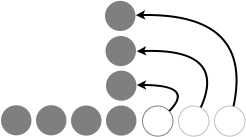
\includegraphics[scale=0.4]{FiguresMaths/SumOddsIntermediate}
              \caption{Folding a single row into a reversed letter ``$L$''.}
       \label{fig:sumOdds2}
\end{center}
\end{figure}

Once we have folded every row of bullets into a reversed ``$L$'', we
nest the occurrences of ``$L$'' in the manner depicted in
Fig~\ref{fig:sumOdds3}.
\begin{figure}[ht]
\begin{center}
       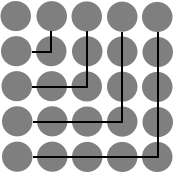
\includegraphics[scale=0.4]{FiguresMaths/SumOddsFinal}
\caption{The final picture organized as an $n \times n$ square
  array of bullets.}
       \label{fig:sumOdds3}
\end{center}
\end{figure}
Clearly, this nesting produces an $n \times n$ square array of
(perforce, $n^2$) bullets.
\end{proof}

\medskip

\index{$n^2$ as sum of first $n$ odd integers!another proof ``by pictures''}
\begin{proof}
{\bf Another proof ``by pictures''.}
%
The reader who enjoyed our ``proof 'by pictures''' may be amused by
the challenge of completing the kindred proof that is illustrated by
Fig.~\ref{fig:anotherSumOdds}.
\begin{figure}[ht]
\begin{center}
       
\includegraphics[scale=0.4]{FiguresMaths/Deltaodd}
\caption{Four copies of $S(n)$ represented as a trianle of bullets.
  The triangles are arranged to yield a $2n \times 2n$ square of
  bullets.}
       \label{fig:anotherSumOdds}
\end{center}
\end{figure}
The figure arranges four copies of the triangle of bullets that
illustrates summation $S(n)$ in such a way that the triangles combine
to produce the $2n \times 2n$ square of bullets.  The underlying
arithmetic exposes the fact that the side of the square consists of
$1+2n-1 \ = \ 2n$ bullets.  The conclusion is that $4 S(n) \ =
\ (2n)^2n \ = \ 4n^2$.
\end{proof}

\ignore{********
{\Denis I added the following construction in the 2 figures, please, select the one you prefer.
If you think this result is too marginal here, we can put it as an exercice...}
This result can be obtained similarly by a slightly different arrangement by counting the bullets
of $4$ triangles representing the sum of the first $n$ integers $S(n)$ as shown in Fig~\ref{fig:alternateSumOdds}.
The side of the square is equal to $1+2n-1=2n$, thus $4 \cdot S(n)=(2n)^2= 4n^2$.

%\begin{figure}[ht]
%\begin{center}
%       
\includegraphics[scale=0.4]{FiguresMaths/DeltaoddSynthetic}
%\caption{Schematic view of how to obtain the $2n \times 2n$ square.}
%       \label{fig:alternateSumOdds2}
%\end{center}
%\end{figure}
***************}
\medskip

\index{$n^2$ as sum of first $n$ odd integers!a proof by rearranging terms}
\begin{proof}
{\bf A proof by rearranging terms.}
%
We describe in Section~\ref{sec:Fubini} how the Italian mathematician
Guido Fubini
\index{Fubini, Guido}
%
was able to make notable mathematical progress by rearranging
representations \cite{Fubini}.  Within the context of the current
chapter, such rearrangements work on the terms of a summation of
interest.  Indeed, using this strategy, we obtain a surprising,
delightful proof of Proposition~\ref{thm:squares-odd-integers-Gauss}.
Let us take the odd integers in order, in groups of sizes $1$, then
$2$, then $3$, and so on.  We begin with the first $n$ odd integers in
order:
\[ 1, \ 3, \ 5, \ 7, \ 9, \ 11, \ 13, \ 15, \ 17, \ 19, \ \ldots \]
Now we start peeling off prefixes of successive numbers of odd
integers and arranging them in an array, as depicted in
%Table~\ref{tab:SumOddsTriangle}.
the following table.
\[
\begin{array}{llrrrrclcc}
\mbox{group of size 1:} & &
1,  &    &     &     &  \rightarrow & 1           & = & 1^3 \\
\mbox{group of size 2:} & &
3,  &  5, &     &    &  \rightarrow & 2 \times 4  & = & 2^3 \\
\mbox{group of size 3:} & &
7,  &  9, & 11, &    &  \rightarrow & 3 \times 9  & = & 3^3 \\
\mbox{group of size 4:} & &
13, & 15, & 17, & 19 &  \rightarrow & 4 \times 16 & = & 4^3 \\
\end{array}
\]
What we note is that---at least with the illustrated portion of the
procedure---the $k$th group, of size $k$, adds up to $k^3$.

%\begin{table}[ht]
%\label{tab:SumOddsTriangle}
%\caption{The sums of successive odd numbers and the sum of
%  successive cubes}
%\end{table}

Before we proceed further, let us verify---by induction---that this
pattern persists indefinitely.
\begin{description}
\item[{\sf Base for the induction.}]
The trivial one-term entry in row $1$ of the preceding table
%~\ref{tab:SumOddsTriangle}
provides the base for our induction.

\medskip

\item[{\sf Inductive hypothesis}.]
We know from Proposition~\ref{thm:sum-first-integers-Gauss} that the
$k$th group consists of $k$ consecutive odd numbers beginning with
\[ 2 \Delta_{k-1} +1 \ \ \ \ \
\mbox{which is the} \ \ \ \ \
\left( \Delta_{k-1} +1 \right)\mbox{th odd number}
\]
Hence, this group begins with $2 \Delta_{k-1} +1$ and ends with
$2\Delta_k -1$.
%{\Denis the right expression is: beginning with $2\Delta_{k-1} +1$ and ending at $2\Delta_k-1$}

%{\Denis I prefer to refer to $\Delta_k$ instead of ${k+1 \choose 2} $... }

This proof can be represented graphically as follows.  We begin with
the unit square (the leftmost item in Fig.~\ref{fig:sumCubes1}) as the
basis of our induction.
\begin{figure}[ht]
\begin{center}
       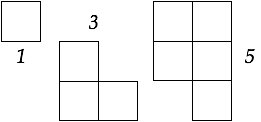
\includegraphics[scale=0.4]{FiguresMaths/SumCubes1}
\caption{The basis for the inductive pictorial proof}
       \label{fig:sumCubes1}
\end{center}
\end{figure}
We next represent the number $2^3$ (the {\em cube} of $2$) by two $2
\times 2$ squares: the figures following the unit square in
Fig.~\ref{fig:sumCubes1}.
\begin{figure}[ht]
\begin{center}
       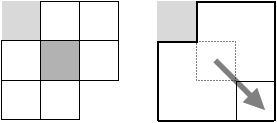
\includegraphics[scale=0.4]{FiguresMaths/SumCubes2}
\caption{Showing graphically that $2^3 +1$ is a perfect square}
       \label{fig:sumCubes2}
\end{center}
\end{figure}
Fig.~\ref{fig:sumCubes2} illustrates graphically that $1+ 2^3$
is a perfect square.
\begin{figure}[ht]
\begin{center}
       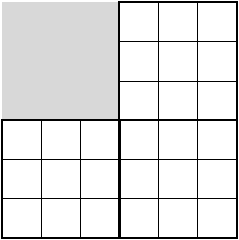
\includegraphics[scale=0.4]{FiguresMaths/SumCubes3}
\caption{The next step in the construction also produces a perfect square}
       \label{fig:sumCubes3}
\end{center}
\end{figure}
Fig.~\ref{fig:sumCubes3} illustrates that iterating the process also
produces a perfect square.  Comparing Figs.~\ref{fig:sumCubes2}
and~\ref{fig:sumCubes3} indicates a parity constraint on the process:
at even-numbered steps,the subsquares that get ``merged'' are
overlapping; at odd-numbered steps, they are not.

\medskip

\item[{\sf Inductive extension}.]
%
Since successive odd numbers differ by $2$, we know that the $k$th
group consists of the following odd integers ($k>1$):
\[
2 \Delta_{k-1} +1, \ 2 \Delta_{k-1}  +3, \ 2 \Delta_{k-1}  +5 ,
\ldots, \
2 \Delta_{k-1} + (2k-1)
\]
Once one verifies (say, by induction) that $2 \Delta_{k-1} +2k-1 \ = \ 2
\Delta_{k} +1$, one discovers that this group has the sum
\[
2k \Delta_{k-1} \ - \ 2 \Delta_{k-1} +k \ = \
(2k -1) \Delta_k + k \ = \ k^3.
\]
\end{description}

%{\Denis here is my solution... Please, check}

Because each row contains one more integer than its predecessor, row
$k$ contains the sum of the odd integers from $\Delta_{k-1}+1$ to
$\Delta_k$.  By direct calculation, we can therefore compute the row's
sum as
\[
\Delta_k^2 \ - \ \Delta_{k-1}^2 
%\left( \frac{k(k+1)}{2} \right)^2 \ - \ \left( \frac{k(k-1)}{2} \right)^2
 \ \ =  \ \ \frac{k^2}{4} \left( (k+1)^2 - (k-1)^2 \right)
% & = & \frac{k^2}{4} (4k) \\
 \ \ = \ \ k^3
\]
\end{proof}

\bigskip

We close our treatment of
Proposition~\ref{thm:squares-odd-integers-Gauss} with another, really
basic proof.  As stated earlier, our goal is really to encourage
readers to utilize every possible mathematical concept as they hone
their mathematical and computational skills: {\em Simple proofs often
lend as much insight as sophisticated ones.}

\medskip

\index{$n^2$ as sum of first $n$ odd integers!a proof from elementary school}
\begin{proof}
{\bf A final proof, from elementary school.}
%
Consider the following reasoning which emerges from the way
multipication tables are developed in elementary school.  We
illustrate the idea using the case $n=5$.
\[
\begin{array}{rrrrr}
1  &  2 &  3 &  4 &  5 \\
2  &  4 &  6 &  8 & 10 \\
3  &  6 &  9 & 12 & 15 \\
4  &  8 & 12 & 16 & 20 \\
5  & 10 & 15 & 20 & 25 \\
\end{array}
\]
Write the integers $1, 2, \ldots, n$ in a row.  Below this row, write
the doubles of these integers.  Below the ``double'' row, write the
triples of the integers.  Below the ``triple'' row, write the
quadruples of the integers, then the quintuples, and so on.  Note that
the resulting table is symmetric: its rows are identical to its
columns.

Using Fubini's rearrangement stratagem, we count all the integers in
the table in two different ways.
\begin{enumerate}
\item
We sum the entries of our table by peeling away successively larger
reversed instances of the letter ``$L$'' (as in our earlier
``pictorial'' proof of
Proposition~\ref{thm:squares-odd-integers-Gauss}).  We find that the
integers in each ``$L$'' sum to a perfect cube:
\[
\begin{array}{ccccccccc|cl}
1  &    &    &    &    &   &     &    &   & 1   & = 1^3 \\
2  &  4 &  2 &    &    &   &     &    &   & 8   & = 2^3 \\
3  &  6 &  9 &  6 &  3 &   &     &    &   & 27  & = 3^3 \\
4  &  8 & 12 & 16 & 12 &  8 &  4 &    &   & 64  & = 4^3 \\
5  & 10 & 15 & 20 & 25 & 20 & 15 & 10 & 5 & 125 & = 5^3
\end{array}
\]

\item
We sum the successive rows of our previous $n$ by $n$ table.  The
first row of the table sums to $\Delta_n$; the second sums sums to $2
\Delta_n$; the third sums to $3 \Delta_n$, \ldots; the last row sums
to $n \Delta_n$.  Thus, the total sum is $(1 + 2 + \cdots + n)
\Delta_n \ = \ \left(\Delta_n \right)^2$.
\end{enumerate}
We conclude that
\[
\sum_{i=1}^n i^3 \ = \  \left(\Delta_n \right)^2
\]
\end{proof}

\ignore{\Arny More calculation!  BOO!  Please complete this.  I seem to be off by 1}
%We give another proof that tells us something more on numbers of their interactions.
%We consider numbers instead of bullets, and we use a similar principle as Fubini, that is to determine a
%suitable organization of the numbers and count them in a simple way.
%For the concern of computing the sum of the first odd numbers, we organize them as shown in Table~\ref{tab:SumOddsTriangle}.
%One number in the first row, two in the second, $k$ on the $k$th row.
%There are $\Delta_p$ (complete) rows. 
%The result is obtained by summing up the elements of each row.
%The sum in a row is equal to the perfect cube of this row.
%This result can be easily proven. 
%{\Denis Should I develop here? or we can let it as an exercice?}
%

\bigskip

{\it A promise, as we close the section.}
%
In Section~\ref{sec:sum-of-i2c>0}, we develop the underpinnings of
techniques that incrementally compute the sums of the first $n$
consecutive integers (the summations $S_1(n)$), the squares of these
integers (the summations $S_2(n)$), the cubes of these integers (the
summations $S_3(n)$), and so on.  Most interesting are the
techniques that are incremental, i.e., that compute the summations
$S_c(n)$ for $c$th powers of integers from the summations for
smaller powers: $S_1(n)$, $S_2(n)$, \ldots, $S_{c-1}(n)$.

\bigskip

\paragraph{\sf C. A nonobvious identity for arithmetic sums}
%
We close this subsection by using a ``picture'' to verify an identity for
arithmetic sums that one would be unlikely to come upon by purely
textual thinking.

\begin{prop} 
\label{thm:an-arithmetic-identity}
For any positive integer $n$,
\[ \Delta_{2n-1} \ = \ n + 4 \Delta_{n-1}. \]
\end{prop} 

\begin{proof} 
Consider the arithmetic series in (\ref{eq:arith-seq}) for the case
$a=1$ and $b=4$.  By Proposition~\ref{thm:sum-of-arithmetic-series},
this series, call it $S^{(1,4)}(n)$, has the sum
\begin{equation}
\label{eq:triangles}
S^{(1,4)}(n) \ = \ n + 4 \Delta_{n-1}.
\end{equation}

Let us represent the sum $\Delta_{n-1}$ in the natural way as a
triangle of bullets.  This triangle has a base of $n-1$ bullets, upon
which sits a row of $n-2$ bullets, upon which sits a row of $n-3$
bullets, \ldots, all the way to the apex, which has a single bullet.

Now, let us view equation (\ref{eq:triangles}) as giving us access to four
copies of the preceding triangle of bullets.  Let us arrange these
triangles in the manner depicted in Fig.~\ref{fig:Delta(n)4}.
\begin{figure}[ht]
\begin{center}
       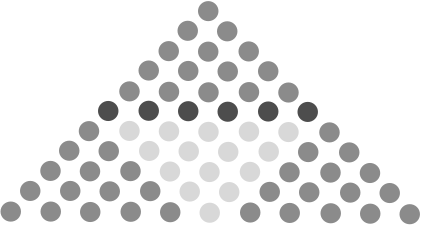
\includegraphics[scale=0.5]{FiguresMaths/Delta4}
 \caption{Arranging the four triangles plus a row to obtain a new (bigger) triangle.}
       \label{fig:Delta(n)4}
\end{center}
\end{figure}
Now, ``complete the picture'' by adding an ``extra'' row of $n$
bullets at row $n$ of the figure (these are depicted in dark gray in
the figure).  The four small triangles, augmented by the ``extra'' row
of $n$ bullets has clearly become a representation  of $\Delta_{2n-1}$
by bullets.
\ignore{******
The sum is $S(n)=n+4 \Delta_{n-1}$.  From the arrangement given in
Fig.~\ref{fig:Delta(n)4}, it is easy to see that it is equal to
$\Delta_{2n-1}$ (4 triangles of size $n$ plus a row of $n$ bullets in
dark grey form a bigger triangle of size $2n-1$).
*******}

We now have a purely pictorial proof of the proposition.
\end{proof} 

\begin{quote}
Full disclosure: {\em Our proof of
  Proposition~\ref{thm:an-arithmetic-identity} is not {\em purely}
  pictorial, because we must somehow verify that the construction is
  completely general, i.e., that the depicted emergence of the
  $\Delta_{2n-1}$ triangle of bullets from four copies of the
  $\Delta_n$-triangle plus the extra row of $n$ bullets is not an
  artifact of the depicted case $n =6$.

Even with this caveat, one must admit that the {\em discovery} of the
proposition is really pictorial, even if the verification requires
additional modalities of reasoning. }
\end{quote}

\ignore{***********
{\Arny I vote that we leave this  as an exercise}

{\Denis Here is another result that may be put as an exercice...}
Consider again the sum of the first integers $\Delta_n$. 
We show graphically that $\Delta_n$ is congruent to $1$ modulo $8$.
\begin{figure}[ht]
\begin{center}
       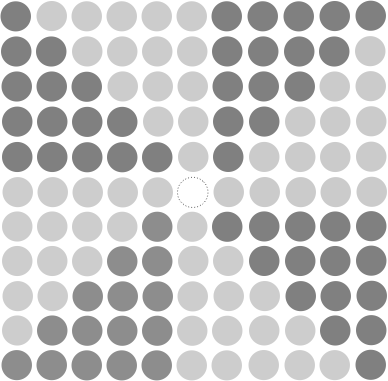
\includegraphics[scale=0.4]{FiguresMaths/Delta8}
\caption{8 copies of $\Delta_n$ are filling a square but one bullet.}
       \label{fig:Sum8deltas}
\end{center}
\end{figure}
****************}
%%%%%%%%%%%%%%%%%%%%%%%%%%%%%%%%%%%%%%%%%%%%%%%%%%%%

\subsection{Geometric Sums and Series}
\label{sec:geometric-sums}
\label{sec:general-geometric-sums}

\subsubsection{Overview and main results}

We define geometric sequences and learn how to calculate their sums
via the following generic examples.
\index{geometric sequence}
\index{geometric summations}
\index{geometric series}

An $n$-term geometric sequence:
\begin{equation}
\label{eq:genl-geom-seq}
a, \ ab, \ ab^2, \ \ldots, ab^{n-1}
\end{equation}

The corresponding geometric summation:
\begin{eqnarray}
\label{eq:genl-geom-summation}
S_{a,b}(n)
 & \eqdef &  \sum_{i=0}^{n-1} a b^i \\
\nonumber
 & = &  a + ab + ab^2 + \cdots + ab^{n-1} \\
\nonumber
 & = & 
 a \cdot (1+ b + b^2 + \cdots + b^{n-1})
\end{eqnarray}

The associated geometric {\em (infinite) series} (used only when $b < 1$):
\begin{equation}
\label{eq:genl-geom-series}
S_{a,b}^{(\infty)} \ \ \eqdef \ \  \sum_{i=0}^\infty a b^i
 \ \  = \ \   a + ab + ab^2 + \cdots 
\end{equation}

It is clear from these definitions that we can evaluate the summation
(\ref{eq:genl-geom-summation}) by evaluating just the sub-summation
\begin{equation}
\label{eq:geom-summation}
S_{b}(n) \ \eqdef \ \sum_{i=0}^{n-1} b^i \ = \
1+ b + b^2 + \cdots + b^{n-1},
\end{equation}
and we can evaluate the series (\ref{eq:genl-geom-series}) by
evaluating just the sub-series
\begin{equation}
\label{eq:geom-series}
S_{b}^{(\infty)} \ \ \eqdef \ \ \sum_{i=0}^\infty b_i \ \ = \ \
1+ b + b^2 + \cdots 
\end{equation}

\medskip

The major results that we develop in this section are:

\index{evaluating geometric sums and series}
\begin{prop}
\label{thm:sum-finite-geometric-series}
Let $S_{b}(n)$ be a geometric summation, as defined in
(\ref{eq:geom-summation}).

\noindent {\bf (a)}
When $b > 1$, $S_{b}(n)$ evaluates to the following sum.
\begin{equation}
\label{eq:geom-sum:b>1}
S^{(b>1)}_{b}(n) \ = \ \frac{b^{n}- 1}{b - 1}.
\end{equation}

\noindent {\bf (b)}
When $b < 1$, $S_{b}(n)$ evaluates to the following sum.
\begin{equation}
\label{eq:geom-sum:b<1}
S^{(b<1)}_{b}(n) \ = \ \frac{1 - b^n}{1-b}.
\end{equation}
\end{prop}

Of course, in the uninteresting degenerate case $b=1$
\[ S^{(b=1)}_{b}(n) \ = \ 1 + 1 + \cdots + 1 \ \ \ \mbox{($n$ times)}
  \ \ \ \ = \ n.  \]

\medskip

The infinite case (\ref{eq:geom-series}) can be dealt with as a
corollary to Proposition~\ref{thm:sum-finite-geometric-series}(b), by
letting $n$ grow without bound and observing that the resulting
sequence of values converges.

\begin{prop}
\label{thm:sum-infinite-geometric-series}
When $b < 1$,  the {\em infinite} series $S^{(\infty)}_{b}$ {\em
  converges} to the following sum.
\[ S^{(\infty)}_{b} \ \ = \ \
\sum_{i=0}^\infty \ b^i \ \ = \ \ 1 + b + b^2 + \cdots
 \ \ = \ \ \frac{1}{1-b}.
\]
\end{prop}

\subsubsection{Techniques for summing geometric series}
\label{sec:summing-geometric-series:techniques}

We turn now to a sequence of proofs of
Propositions~\ref{thm:sum-finite-geometric-series}
and~\ref{thm:sum-infinite-geometric-series}.

\medskip

\index{evaluating geometric sums and series!by textual replication}
\begin{proof}
{\bf A proof by textual replication.}
%
Toward the end of developing our first method for summing $S_{b}(n)$,
we note that we can rewrite the sum in two ways that are {\em
  (textually) recurrent}.

\bigskip

\noindent
{\em This phenomenon of {\em finding recurrent subexpressions} is a
  ``pattern'' of the form described in Section~\ref{sec:manifesto} as
  we discussed how mathematicians ``do mathematics''.  We now
  exemplify how this pattern can be exploited to find explicit sums
  for geometric summations and series.}

\bigskip

\noindent
Both of the recurrent expressions for $S_{b}(n)$ have the following form.
\begin{equation}
\label{eq:geom-series-recurrent}
S_b(n) \ = \ \alpha \cdot S_b(n) \ + \ \beta(n)
\end{equation}
where $\alpha$ is a constant and $\beta(n)$ is a function of $n$; both
$\alpha$ and $\beta(n)$ may depend on the parameter $b$.  We provide
two recurrent expressions for $S_b(n)$, one of which is more
interesting when $b>1$, the other when $b<1$.
\begin{eqnarray}
\label{eq:geom-series-replicate}
\nonumber
S_{b}(n) 
  & \eqdef &
1+ b + b^2 + \cdots + b^{n-1}  \\
\nonumber
  &   &  \\
\label{eq:geom-series-replicate-1}
%  & = & 1 + b \cdot S_{b}(n) - b^n
   & = & b \cdot S_{b}(n) \ + \ (1 - b^n) \\
\nonumber
   &  & \\
%  & = & {\displaystyle
%b^{n-1} + \frac{1}{b} \cdot S_{b}(n) - \frac{1}{b}}
\label{eq:geom-series-replicate-2}
  & = &
\frac{1}{b} \cdot S_{b}(n) \ + \ \frac{b^n -1}{b} 
\end{eqnarray}
The significance of a recurrent expression of the form
(\ref{eq:geom-series-recurrent}) is that it exposes an explicit value
for $S_b(n)$:
\begin{equation}
\label{eq:geom-series-generic}
S_b(n) \ = \ \frac{\beta(n)}{1 - \alpha}
\end{equation}

We now combine the generic value (\ref{eq:geom-series-generic}) of
$S_b(n)$ with the specialized recurrent expressions in
(\ref{eq:geom-series-replicate-1}) and
(\ref{eq:geom-series-replicate-2}) to derive two explicit solutions
for $S_b(n)$.
\begin{enumerate}
\item
The first solution is most useful and perspicuous when $b>1$.  In this
case, we find that
\[ \left( 1 - \frac{1}{b} \right)  S^{(b>1)}_{b}(n) \ = \ b^{n-1} -
\frac{1}{b}, \]
which can easily be rearranged to the equivalent and more
perspicuous form (\ref{eq:geom-sum:b>1}).

\item
The second solution is most useful and perspicuous when $b < 1$.  In this
case, we find that
\[ (1-b) S^{(b<1)}_{b}(n) \ = \ 1 \ - \ b^n \]
which can easily be rearranged to the equivalent and more
perspicuous form (\ref{eq:geom-sum:b<1}).
\end{enumerate}
\end{proof}

Note that both $S^{(b>1)}_{b}(n)$ and $S^{(b<1)}_{b}(n)$ have simple
{\em approximate} values which are useful in ``back-of-the-envelope''
calculations: For very large values of $n$, we have
\begin{equation}
\label{eq:geom-sum:approx}
S^{(b>1)}_{b}(n) \ \approx \ \frac{b^n}{b-1} \ \ \
\mbox{and} \ \ \
S^{(b<1)}_{b}(n) \ \approx \ \frac{1}{1-b} .
\end{equation}
The expression for $S^{(b<1)}_{b}(n)$ in (\ref{eq:geom-sum:approx}) is
actually a rewording of
Proposition~\ref{thm:sum-infinite-geometric-series}.

\medskip

\index{evaluating geometric sums and series!a pictorial way to sum
  $S^{(\infty)}_{1/2}$ using cascading shrinking squares}
\begin{proof}
{\bf A pictorial representation for summing $S^{(\infty)}_{1/2}$.}
%
Fig.~\ref{fig:sumGeoBasis} depicts a pictorial process whose analysis
provides a rigorous proof of
Proposition~\ref{thm:sum-infinite-geometric-series} for the case $b =
1/2$, \textit{i.e.}, a rigorous argument that the series $S^{(\infty)}_{1/2} =
\sum_{i=0}^\infty \ 2^{-i}$ sums to $2$.
\begin{figure}[ht]
\begin{center}
       \includegraphics[scale=0.4]{FiguresMaths/SumGeometric1sur2Bis}
 \caption{Arranging successive rectangles to evaluate $S^{(\infty)}_{1/2}$.}
       \label{fig:sumGeoBasis}
\end{center}
\end{figure}
In this evaluation of $S^{(\infty)}_{1/2}$, we measure fractional
quantities by the portion of a unit-side rectangle that they fill.
Thus (follow in the figure): the initial term of $S^{(\infty)}_{1/2}$,
namely $1$, is represented by the unit square that is labeled ``$1$''
in the figure.  The next term of the series, namely $1/2$, is
represented by the rectangle labeled ``$1/2$'' in the figure, and so
on, with successively smaller rectangles.  By designing each rectangle
to have half the area of its predecessor, the sequence of rectangles
thus represents successively smaller inverse powers of $2$.  As the
process proceeds, we observe increasingly more of the righthand
unit-side square being filled.  In fact, one can argue that {\em
  every} point in the righthand unit-side square eventually gets
covered by some small rectangle (as $n$ tends to $\infty$), thereby
establishing that the infinite series $S^{(\infty)}_{1/2}$
does, indeed, sum to $2$.

\ignore{*******
The result is immediate while considering a basic unit square and its
successive decompositions while divided by $2$.
Thus, the whole surface corresponds to the sum of $(\frac{1}{2})^k$. 
It is equal to $2$ (surface of the two big squares) and it is completely filled. 
***********}

This procedure is difficult, but not impossible, to adapt to values of
$b <1$ other than $1/2$.  The sequence Fig.~\ref{fig:sumGeoGeneral1},
\begin{figure}[ht]
\begin{center}
       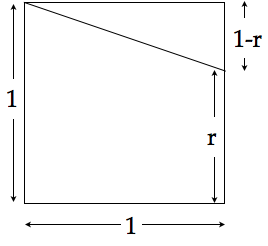
\includegraphics[scale=0.4]{FiguresMaths/SumGeometricGeneral1}
\caption{Initial state: the unit square and the base $b$.}
       \label{fig:sumGeoGeneral1}
\end{center}
\end{figure}
Fig.~\ref{fig:sumGeoGeneral2},
\begin{figure}[ht]
\begin{center}
       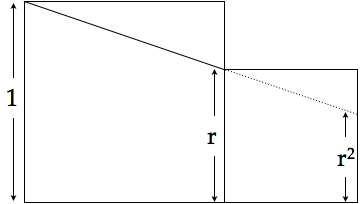
\includegraphics[scale=0.4]{FiguresMaths/SumGeometricGeneral2}
\caption{Beginning to craft the geometric series by cascading
  shrinking squares.}
       \label{fig:sumGeoGeneral2}
\end{center}
\end{figure}
Fig.~\ref{fig:sumGeoGeneral3} suggests how to achieve such an
adaptation for any value of $b$ with $0 \leq b <1$, by an
appropriate cascade of shrinking squares.
\begin{figure}[ht]
\begin{center}
       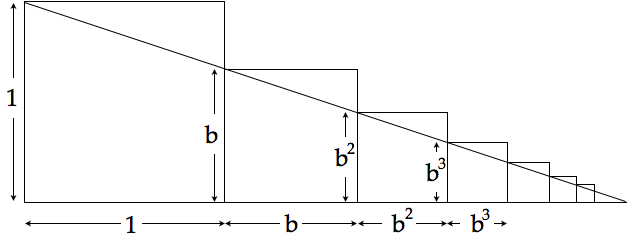
\includegraphics[scale=0.4]{FiguresMaths/SumGeometricGeneral3}
\caption{The complete process for computing a geometric series using a
  cascade of shrinking squares.}
       \label{fig:sumGeoGeneral3}
\end{center}
\end{figure}
The unit-side square in Fig.~\ref{fig:sumGeoGeneral1} begins the
construction of the cascade.  The two squares in
Fig.~\ref{fig:sumGeoGeneral2} illustrate the second step in
constructing the cascade; the suggestive cascade depicted in
Fig.~\ref{fig:sumGeoGeneral3} illustrates what the final cascade looks
like: the cumulative length of the bases of its abutting rectangles is
the value of the infinite series $S^{(\infty)}_{b} =
\sum_{i=0}^\infty \ b^{i}$ (where $0 \leq b < 1$).
\end{proof}

\medskip

%{\Denis We can add here two exercices.}
\ignore{************
{\Denis(1) I really like including the pie-cutting in the text,
  because it is another representation for exactly the same problem.
  Do you like this way of handling it?  
  YES
  (2) I am less enthusiastic
  about including the nexted triangles: it changes the problem (i.e.,
  the base b) as well as the representation.  
  OK, basie b is somehow a generalization...
  I like it very much as
  an exercise ... but we have not yet tackled that issue.
  How the exercices will be included?}
**********}

\index{evaluating geometric sums and series!a pictorial way to sum
  $S^{(\infty)}_{1/2}$ using a vigorously sliced pie}
\begin{proof}
{\bf Another pictorial representation for summing $S^{(\infty)}_{1/2}$.}
%
The pictorial derivation of the sum $S^{(\infty)}_{1/2}$ can be
accomplished using geometric shapes other than squares.  We now
present a natural derives the sum $S^{(\infty)}_{1/2}$ by vigorously
slicing a pie.

The process of pie-slicing works most naturally with the modified
series
\[ \overline{S}^{(\infty)}_{1/2} \ \ = \ \ \sum_{i=1}^\infty 2^{-i}
 \ \ = \ \ S^{(\infty)}_{1/2} \ - \ 1. \]
which omits the initial summand $1$ from $S^{(\infty)}_{1/2}$.  Of
course, $\overline{S}^{(\infty)}_{1/2}$ sums to $1$, because
$S^{(\infty)}_{1/2}$ sums to $2$.

The pie-slicing evaluation of $\overline{S}^{(\infty)}_{1/2}$ is depicted
in Fig~\ref{fig:sumGeo1sur2circle}.  In the figure, the inverse powers
of $2$ are represented by appropriate fractions of a unit-diameter
disk (the pie).  The evaluation begins with this disk before it is
sliced: this represents the number $1$, which we eventually show to be
the sum of $\overline{S}^{(\infty)}_{1/2}$.
\begin{figure}[ht]
\begin{center}
       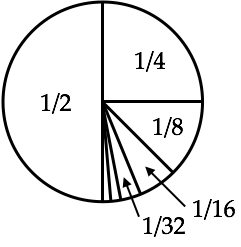
\includegraphics[scale=0.4]{FiguresMaths/SumGeometric1sur2circle}
\caption{Computing the sum of $1/2^i$ using a unit disk.}
       \label{fig:sumGeo1sur2circle}
\end{center}
\end{figure}
We slice the disk in half by means of the depicted diameter; we label
one of the resulting half-disks ``$1/2$''.  Next, we slice one of the
half-disks in half by means of a radius of the unit disk; we label one
of the quarter-disks ``$1/4$''.  We continue in this manner {\em ad
  infinitum}.  The analysis that yields the sum of
$\overline{S}^{(\infty)}_{1/2}$ amounts to a proof that every point in the
unit-diameter disk eventually resides in a slice that is not further
sliced.  Details are left to the interested reader.
\end{proof}

\ignore{***************
Another variation refers to the surface of an unit equilateral triangle. 
We are looking for the sum of the $1/4^i$ is equal to $1/3$ by two ways
refering to Fig~\ref{fig:sumGeo1sur4}: The area of the infinite sum represented in dark grey is obviously one third of the total area
(easy to see if we remark that the dark triangles are one third in each layer...). 
\begin{figure}[ht]
\begin{center}
       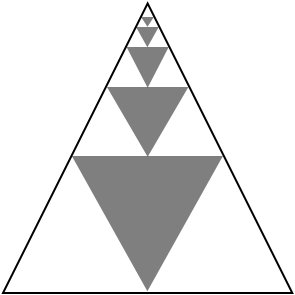
\includegraphics[scale=0.4]{FiguresMaths/SumGeometric1sur4}
\caption{Computing the sum of $1/4^i$.}
       \label{fig:sumGeo1sur4}
\end{center}
\end{figure}
******************}

\subsubsection{A fun result via geometric sums: When is integer  $n$
  divisible by $9$?}
\label{sec:divisible-by-9}

We now exploit our ability to evaluate geometric summations to
illustrate a somewhat surprising, nontrivial fact.  One can deduce
information about the divisibility of an integer $n$ from $n$'s
positional numerals.  We hope that this ``fun'' result will inspire
the reader to seek kindred numeral-encoded properties of numbers.

\begin{prop}
\label{thm:div-by-b-bar}
An integer $n$ is divisible by an integer $m$ if, and only if, $m$
divides the sum of the digits in the base-$(m+1)$ numeral for $n$.
\end{prop}

The most familiar instance of this result is phrased in terms of our
traditional use of base-$10$ (decimal) numerals. \\
{\it An integer $n$ is divisible by $9$ if, and only if, the sum of
  the digits of $n$'s base-$10$ numeral is divisible by $9$.}

\smallskip

\begin{proof}
({\it Argument for general number-base $b$}).
%
Of course, we lose no generality by focusing on numerals without
leading $0$'s, because leading $0$'s do not alter a numeral's sum of
digits.

Let us focus on the base-$b$ numeral for a number $n$ (so $b = m+1$ in
the statement of the proposition).  There therefore exist base-$b$
digits---i.e., integers from the set $\{0, 1, \ldots, b-1\}$---call
them $\delta_k \neq 0$, $\delta_{k-1}$, \ldots $\delta_1$, $\delta_0$,
such that
\[ n \ = \ \delta_k \cdot b^k + \delta_{k-1} \cdot b_{k-1} + \cdots +
\delta_1 \cdot b + \delta_0. \]
The sum of the digits of $n$'s base-$b$ numeral is, then
\[ s_b(n) \ \eqdef \ \delta_k + \delta_{k-1} + \cdots + \delta_1 +
\delta_0. \]
Let us calculate the difference $n - s_b(n)$ in the following manner,
digit by digit.
\begin{equation}
\label{eq:sum-of-digits}
\begin{array}{ccccccccccc}
n & = &
\delta_k \cdot b^k & + & \delta_{k-1} \cdot b^{k-1} & + & \cdots
  & + & \delta_1 \cdot b & + & \delta_0 \\
s_b(n) & = &
\delta_k & + & \delta_{k-1} & + & \cdots & + & \delta_1 & + & \delta_0 \\
\hline
n - s_b(n) & = &
\delta_k \cdot (b^k -1) & + &
\delta_{k-1} \cdot (b^{k-1} -1) & + &
\cdots & + &
\delta_1 \cdot (b-1) & & 
\end{array}
\end{equation}

\medskip

We now revisit summation (\ref{eq:geom-sum:b>1}).  Because $b$ is a
positive integer, so that $1 + b + \cdots + b^{a-2} + b^{a-1}$ is also
a positive integer, we infer that {\em the integer $b^a -1$ is
  divisible by $b-1$.}

We are almost home.  Look at the equation for $n - s_b(n)$ in the
system (\ref{eq:sum-of-digits}).  As we have just seen, every term on
the righthand side of that equation is divisible by $b-1$.  It follows
therefore, that the lefthand expression, $n - s_b(n)$, is also
divisible by $b-1$.
An easy calculation, which we leave to the reader, now shows that this
final fact means that $n$ is divisible by $b-1$ if, and only if,
$s_b(n)$ is.
\end{proof}

\subsubsection{Extended geometric series and their sums}
\label{sec:extended-geom-series}
\index{extended geometric sums: $\sum_{i=1}^n \ i^c b^i$}

We now build on our ability to evaluate geometric summations of the
forms (\ref{eq:geom-sum:b>1}, \ref{eq:geom-sum:b<1}) to evaluate
summations that we shall term {\em extended} geometric summations (not
a standard term), \textit{i.e.}, summations of the form
\[ S_b^{(c)}(n) \ \eqdef \ \sum_{i=1}^n \ i^c b^i, \]
where $c$ is an arbitrary fixed positive integer, and $b$ is an
arbitrary fixed real number.

We restrict attention here to the situation defined by the joint
non-equalities $c \neq 0$ and $b \neq 1$.
\begin{itemize}
\item
We have already adequately studied the case $c=0$, which characterizes
``ordinary'' geometric summations.
\item
The case $b = 1$ removes the ``geometric growth'' of the sequence
underlying the summation.  We study various aspects of this {\it
  summation-of-fixed-powers} case in Section~\ref{sec:smooth-series},
with special treatment of summations of fixed powers of consecutive
integers in Section~\ref{sec:sum-of-i2c}.
\end{itemize}

The method we now develop for evaluating all other summations
$S_b^{(c)}(n)$, \textit{i.e.}, those with $b \neq 1$ and $c \neq 0$, has two
major characteristics.
\begin{enumerate}
\item
The method is {\em inductive in parameter} $c$, in the sense that we
will be able to express our sum for $S_b^{(c)}(n)$ in terms of sums
for summations $S_b^{(c-1)}(n)$, $S_b^{(c-2)}(n)$, \ldots,
$S_b^{(1)}(n)$, $S_b^{(0)}(n) = S_b(n)$.  And, for each fixed value of
$c$, the method is {\em inductive in the argument} $n$.

%{\Denis I am not  so clear here, is it an induction on c or on n? We develop for n  later on...}

\item
The method will rely on the recurrent-subexpression strategy which was so
effective in Section~\ref{sec:general-geometric-sums}.
\end{enumerate}

\medskip

\index{extended geometric sums: $\sum_{i=1}^n \ i^c b^i$!the case $c=1$}
\paragraph{\sf A. The extended geometric sum $S^{(1)}_b(n) = \sum_{i=1}^n
  i b^i$}
We illustrate our strategy in detail for the case $c=1$ and sketch
only briefly how it deals with larger values of $c$.  Elementary
algebraic manipulations which are suggested by the analysis in the
case $c=1$ should thereby allow the reader to deal with any value $c >
1$.

\begin{prop}
\label{thm:sum-i2i}
For all bases $b > 1$,
\begin{equation}
\label{eq:sum-i2i}
S_b^{(1)}(n) \ \ = \ \
\sum_{i=1}^n \ i b^i
\ \ = \ \ 
\frac{(b-1)n -1}{(b-1)^2} \cdot  b^{n+1} \ + \ \frac{b}{(b-1)^2}
\end{equation}
\end{prop}

\index{extended geometric sums: $\sum_{i=1}^n \ i^c b^i$!the case
  $c=1$!summing via algebraic manipulation}
\begin{proof}
{\bf Deriving a sum via algebraic manipulation.}
%
We begin to develop our strategy by writing the natural expression for
\[ S_b^{(1)}(n) \ \ = \ \ b \ + \ 2b^2 \ + \ 3 b^3 \ + \cdots + \ n b^n  \]
in two different ways.  First, we isolate the summation's last term:
\begin{equation}
\label{eq:ext-geom-c=1.1}
S_b^{(1)}(n+1) \ = \ S_b^{(1)}(n) \ + \ (n+1) b^{n+1}.
\end{equation}
Then we isolate the summation's first term:
\begin{eqnarray}
\nonumber
S_b^{(1)}(n+1)
     & = &
b + \sum_{i=2}^{n+1} \ i b^{i}  \\
\nonumber
& = &
b + \sum_{i=1}^n \ (i+1) b^{i+1}  \\
\nonumber
     & = &
b +  b \cdot \sum_{i=1}^n \ (i+1) b^i \\
\nonumber
     & = &
b + 
b \cdot \left(
\sum_{i=1}^n \ i b^i 
 \ + \
\sum_{i=1}^n \  b^i 
\right) \\
\nonumber
     & = &
b \cdot \left( S_b^{(1)}(n) \ + \ S_b^{(0)}(n) \right) \ + \ b \\
\nonumber
& = &
b \cdot \left( S_b^{(1)}(n) \ +  \frac{b^{n+1} -1}{b-1} -1 \right) \ + \ b \\
\label{eq:ext-geom-c=1.2}
    & = &
b \cdot S_b^{(1)}(n) \ + \ b \cdot \frac{b^{n+1} - 1}{b-1}
\end{eqnarray}
Combining expressions (\ref{eq:ext-geom-c=1.1}) and
(\ref{eq:ext-geom-c=1.2}) for $S_b^{(1)}(n+1)$, we
finally find that
\begin{eqnarray}
\nonumber
(b-1) \cdot S_b^{(1)}(n) & = &
(n+1) \cdot b^{n+1} \ - \ b \cdot \frac{b^{n+1} -1}{b-1} \\
\label{eq:sum-i2i-source}
 & = &
\left( n - \frac{1}{b-1} \right) \cdot b^{n+1} \ + \ \frac{b}{b-1}
\end{eqnarray}
One now uses standard algebraic manipulations to derive expression
(\ref{eq:sum-i2i}) from equation (\ref{eq:sum-i2i-source}).
%so that, finally,
%\[ S_b^{(1)}(n) \ = \
%\frac{bn -n -1}{(b-1)^2} \cdot  b^{n+1} \ - \ \frac{b}{(b-1)^2}
%\]
\end{proof}

%{\Denis I add below a particular case,
%I think this is really interesting since it illustrates another technique of switching the indices in double sums}

\index{extended geometric sums: $\sum_{i=1}^n \ i^c b^i$!the case
  $c=1$!solving the case $b=2$ using subsum rearrangement}
\begin{proof}
{\bf Solving the case $b=2$ using subsum rearrangement.}
%
We can evaluate the sum
\[
S_2^{(1)}(n) \ = \ \sum_{i=1}^n \ i 2^i
\]
in an especially interesting way, by rearranging the sub-summations of
the target summation.
\begin{quote}
{\em
The reader should pay careful attention to this technique.  It can
sometimes decompose a cumbersome expression for a summation into a
readily manipulated one.
}
\end{quote}
Note that we can rewrite summation $S_2^{(1)}(n)$ as a {\em double
  summation:}
\begin{equation}
\label{eq:geom-double-sum}
S_2^{(1)}(n) \ = \ \sum_{i=1}^n \ \sum_{k=1}^{i} 2^i
\end{equation}

By suitable applications of the laws of arithmetic
Section~\ref{sec:Arithmetic-Laws}---specifically, the distributive,
associative, and commutative laws---we can perform the required double
summation in a different order than that specified in
(\ref{eq:geom-double-sum}).  In fact, we can exchange the indices of
summation, to compute $S_2^{(1)}(n)$ as specified via the following
expression:
\[
S_2^{(1)}(n) \ = \ \sum_{k=1}^{n} \ \sum_{i=k}^{n} 2^i.
\]
This process is illustrated in Fig.~\ref{fig:Sumi2i}.
\begin{figure}[htb]
\centerline{
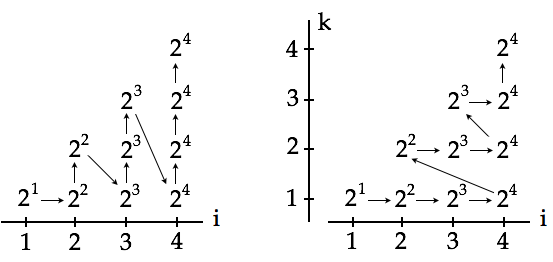
\includegraphics[scale=0.4]{FiguresMaths/Sumi2i}
}
\caption{Illustration of the exchange of indices in the summation.
The original sum is on the left, each $i \cdot 2^i$ is distributed $i$ times on column $i$.
The second sum is obtained by introducing a new index $k$ and to scan each term of the sum row by row (on the right).
The arrows represent the order of execution.}
\label{fig:Sumi2i}
\end{figure}
The indicated summation is much easier to perform in this order,
because its core consists of instances of the ``ordinary'' geometric
summation $\sum_{i=k}^{n} 2^i$ (see
Proposition~\ref{thm:sum-finite-geometric-series}).  Expanding these
instances, we find finally that
\[
S_2^{(1)}(n) \ = \ \sum_{k=1}^{n} \ (2^{n+1} -1 - \sum_{i=0}^{k-1} \ 2^i).
\]
\[
S_2^{(1)}(n) \ = \ \sum_{k=1}^{n} \ (2^{n+1} - 2^k).
\]
\[
S_2^{(1)}(n)
\ \ = \ \ n \cdot 2^{n+1}\ - ( 2^{n+1} -1) +1
\ \ = \ \ (n-1) \cdot 2^{n+1} +2.
\]
\end{proof}

\smallskip

\paragraph{\sf B. The general extended geometric sum $S^{(c)}_b(n) =
  \sum_{i=1}^n i^c b^i$}
We now develop a strategy that adapts the evaluation of summation
$S_b^{(1)}(n)$ in the proof of Proposition~\ref{thm:sum-i2i} to an
evaluation of the general extended geometric summation
\[
S_b^{(c)}(n) \ \ = \ \ \sum_{i=1}^n \ i^c b^i
 \ \ = \ \
b \ + \ 2^{c} b^2\ + \ 3^{c} b^3 \ + \ \cdots \ + \ n^{c} b^{n}
\]
The strategy is {\em recursive}, in that it computes a value for
$S^{(c)}_b(n)$ from values for $S^{(c-1)}_b(n)$, $S^{(c-2)}_b(n)$,
\ldots, $S^{(0)}_b(n)$.  It proceeds in three steps.

\noindent {\bf Step 1.}
%
As in the case $c=1$, we write summation $S_b^{(c)}(n)$ in two ways.
The expression that embodies the first way isolates the summation's
first term:
\[ S_b^{(c)}(n+1) \ = \ b + \sum_{i=1}^n \ (i+1)^c b^{i+1} \]
The expression that embodies the second way isolates the summation's
last term:
\[ S_b^{(c)}(n+1) \ = \ S_b^{(c)}(n) \ + \ (n+1)^{c} b^{n+1}. \]
By combining these expressions, we find that
\begin{equation}
\label{eq:Sbcn-1}
S_b^{(c)}(n) 
 \ = \
b \cdot \left(
1 \ - \
(n+1)^{c} b^{n} \ + \
 \sum_{i=1}^n \ (i+1)^c b^{i} 
\right)
\end{equation}


\noindent {\bf Step 2.}
%
We next invoke the Restricted Binomial Theorem
(Theorem~\ref{thm:restricted-binomial-thm}) to see that
\[ (i+1)^c \ = \ i^c \ + \ c \cdot i^{c-1} \ + \ {c \choose 2} \cdot
i^{c-2} \ + \cdots + \ {c \choose k} \cdot i^{c-k}  \ + \cdots + \ 1
\]

We use this expansion of $(i+1)^c$, together with multiple
applications of the laws of arithmetic from
Section~\ref{sec:Arithmetic-Laws} to verify that
\begin{eqnarray}
\nonumber
\sum_{i=1}^n \ (i+1)^c b^{i} & = &
S_b^{(c)}(n)
 \ + \ c \cdot S_b^{(c-1)}(n)
 \ + \ {c \choose 2} \cdot S_b^{(c-2)}(n)  \ + \cdots \\
\label{eq:Sbcn-2}
  &  & \cdots + \
{c \choose k} \cdot S_b^{(c-k)}(n)
 \ + \cdots + \
S_b^{(0)}(n)
\end{eqnarray}

\noindent {\bf Step 3.}
%
We finally combine equations (\ref{eq:Sbcn-1}) and (\ref{eq:Sbcn-2})
to discover that
\begin{eqnarray}
\nonumber
(b-1) \cdot S_b^{(c)}(n)
 & = &
(n+1)^{c} b^{n} \ - \
c \cdot S_b^{(c-1)}(n)
 \ - \ {c \choose 2} \cdot S_b^{(c-2)}(n)  \ - \cdots \\
\label{eq:Sbcn-3}
  &  & 
\cdots - \
{c \choose k} \cdot S_b^{(c-k)}(n)
 \ - \cdots - \
S_b^{(0)}(n)
\ - \ 1
\end{eqnarray}

We thus have the promised method of evaluating the extended geometric
summation $S_b^{(c)}(n)$ associated with the fixed power $c$ in terms
of the sums of extended geometric summations associated with smaller
fixed powers.

%%%%%%%%%%%%%%%%%%%%%%%%%%%%%%%%%%%%%%%%%

\section{On Summing ``Smooth'' Series}
\label{sec:smooth-series}

\subsection{Approximate Sums via Integration}
\label{sec:riemann-bounds}

This section illustrates a powerful strategy for obtaining nontrivial
upper and lower bounds on the values of sum, by finding continuous {\em
  envelopes} that bound the discrete summations both above and below.
The areas under the enveloping continuous functions---which we can
calculate via integration---provide the desired bounds on the
summations.

The strategem operates via the following three steps.  Say that we
have a sum
\[ a_1 \ + \ a_2 \ + \ \cdots \ + \ a_n \]
For convenience we use a finite sum for illustration; the stratagem
often works with infinite sums also, as our specific examples
illustrate.

\noindent {\sf Step 1.}
Represent the summands seriatim as abutting unit-width rectangles.  

\noindent
Our generic example has $n$ unit-width rectangles, of respective
heights $a_1$, $a_2$, \ldots, $a_n$.  We describe two special cases,
to help the reader understand how the strategem is applied.
\begin{enumerate}
\item
Figs.~\ref{fig:riemann-n2-1} and~\ref{fig:riemann-n2-2} illustrate our
strategem applied to the summation $S_2(n) = \sum_{i=1}^n i^2$.  In
both figures, we represent $S_2(n)$ by the aggregate area of a
sequence of unit-width rectangles.  The rectangles that represent the
respective addends in this example have respective heights $1$, $4$,
$9$, $16$, $25$, $36$ and $49$.  If we were to extend the figures
rightward (to extend the summation by encompassing more addends
thereby increasing $n$), then the next rectangle would have height
$64$.

The rectangles in Fig.~\ref{fig:riemann-n2-1} are accompanied by a
continuous curve (labeled (a) in the figure) which connects their
upper lefthand corners.
\begin{figure}[htb]
\centerline{
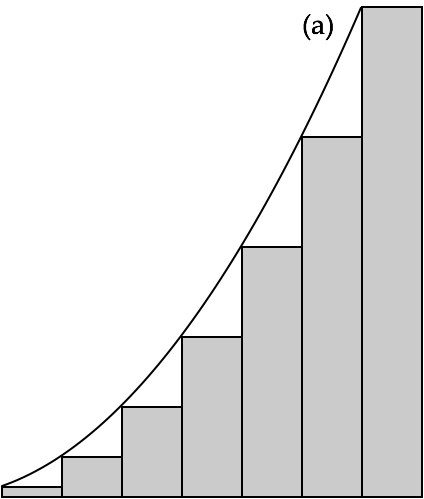
\includegraphics[scale=0.3]{FiguresMaths/SumSquaresContinuous1}
}
\caption{The summation $S_2(n) = \sum_{i=1}^n i^2$ represented by the
  aggregate area of a sequence of unit-width shaded rectangles.  The
  summation is bounded above by the area under the continuous curve (a)
  that connects the upper lefthand corners of the rectangles.  The
  area under curve (a) is $\int_0^n \ (x+1)^2 dx$.  }
\label{fig:riemann-n2-1}
\label{fig:SumIntegral1}
\end{figure}
Because this curve completely ``covers'' the rectangles (which we
emphasize by shading the rectangles), the area under the curve is an
{\em upper bound} on the aggregate area of the rectangles; this area
is
\[ \int_1^n \ x^2 dx \]

The rectangles in Fig.~\ref{fig:riemann-n2-2} are accompanied by a
continuous curve (labeled (b) in the figure) which connects the upper
righthand corners of the rectangles.
\begin{figure}[htb]
\centerline{
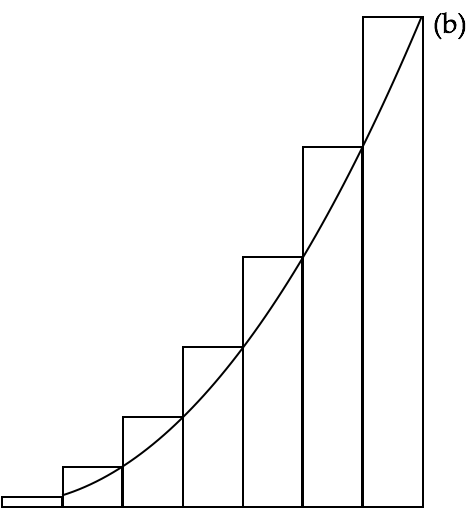
\includegraphics[scale=0.3]{FiguresMaths/SumSquaresContinuous2}
}
\caption{ The summation $S_2(n)$ represented by the aggregate area of
  a sequence of unit-width unshaded rectangles.  The summation is
  bounded from below by the area under the continous curve (b) that
  connects the upper righthand corners of the rectangles.  The area
  under curve (b) is $\int_1^n \ x^2 dx$.}
\label{fig:riemann-n2-2}
%\label{fig:SumIntegral2}
\end{figure}
Because this curve lies completely within the area formed by the
rectangles, the area under the curve is a {\em lower bound} on the
aggregate area of the rectangles; this area is
\[ \int_0^{n-1}  \ \frac{1}{x+1} dx \]

%{\Denis I did with the powers of 2, will change to the squares...}

\item
In Figs.~\ref{fig:riemann-harmonic1} and~\ref{fig:riemann-harmonic2},
we represent the {\em harmonic} sum
\[ S^{(H)}(n) \ = \ \sum_{i=1}^n \ i^{-1} \ = \ \sum_{i=1}^n \ 1/i.
\]
In both figures, $S^{(H)}(n)$ is represented by the aggregate area of
a sequence of abutting unit-width rectangles, of respective heights
$1$, $1/2$, $1/3$, \ldots, $1/10$ (so the figures represent the case
$n=10$).  It would be only a clerical task to add more rectangles, of
heights $1/11$, $1/12$, etc., to represent larger values of $n$.

In Fig.~\ref{fig:riemann-harmonic1}, the rectangles are accompanied by
a continuous curve (marked (a) in the figure) that passes through
their upper righthand corners.
\begin{figure}[htb]
\centerline{
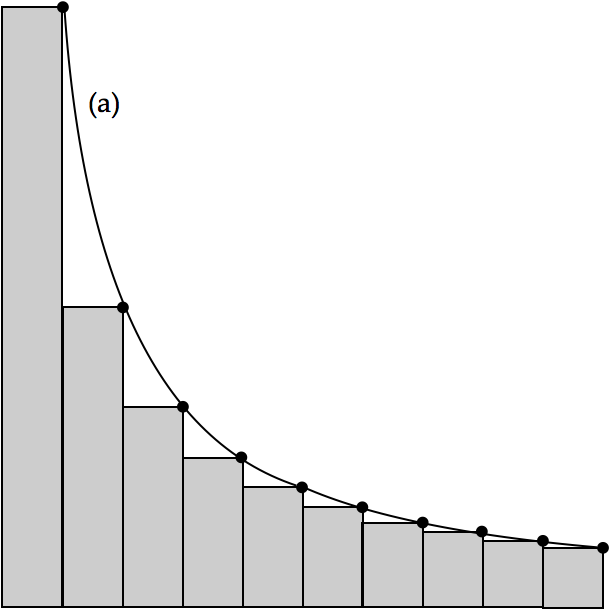
\includegraphics[scale=0.3]{FiguresMaths/RiemannSum1}
}
\caption{The summation $S^{(H)}(n) \ = \ \sum_{i=1}^n \ 1/i$
  represented by the aggregate area of a sequence of unit-width
  rectangles, $S^{(H)}(n)$ is bounded from above by the area under a
  continuous curve (a) that passes through the upper righthand corners
  of the rectangles.  This area is $ \int_1^n \ \frac{1}{x} dx$. }
\label{fig:riemann-harmonic1}
\end{figure}
Because this curve completely ``covers'' the rectangles (which we
emphasize by shading the rectangles), the area under the curve is an
{\em upper bound} on the aggregate area of the rectangles; the area
under curve (a) is
\[ \int_1^n \ \frac{1}{x} dx \]

In Fig.~\ref{fig:riemann-harmonic2}, the rectangles are accompanied by
a continuous curve (marked (b) in the figure) that passes through
their upper lefthand corners.
\begin{figure}[htb]
\centerline{
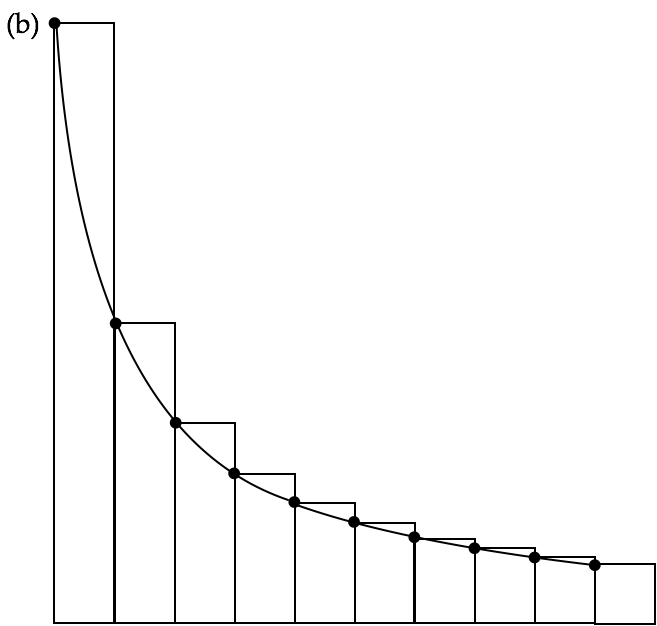
\includegraphics[scale=0.3]{FiguresMaths/RiemannSum2}
}
\caption{Representing the summation $S^{(H)}(n)$ as in
  Fig.~\ref{fig:riemann-harmonic1}, the summation is bounded from
  below by the area under a continuous curve (b) that passes through
  the upper lefthand corners of the rectangles.  The area under curve
  (b) is $\int_0^{n-1} \ \frac{1}{x+1} dx$.}
\label{fig:riemann-harmonic2}
\end{figure}
Because curve (b) lies completely within the aggregate area of the
rectangles, the area under the curve is a {\em lower bound} on the
aggregate area of the rectangles; the area under curve (b) is
\[ \int_0^{n-1}  \ \frac{1}{x+1} dx \]
  \end{enumerate}
%
%{\Denis We should add in the caption the explanation of curves (a) and (b)}
%The rectangles that represent the respective addends have respective
%heights $12$, $6$, $4$, $3$, $16/3$, and $2$.  If we were to extend
%the figure rightward (to extend the summation and encompass more
%addends), then the next rectangle would have height $16/7$.

\medskip

\noindent {\sf Step 2.}
%
Construct a continuous curve $\overline{C}(x)$ that passes through the
corners of the unit-width rectangles specified by the summation, in
such a way that the aggregate areas of the rectangles lies completely
within the area under $\overline{C}(x)$.
\begin{quote}
{\em
The curves labeled (a) in Figs.~\ref{fig:riemann-n2-1}
and~\ref{fig:riemann-harmonic1} are instances of the mandated
continuous curve $\overline{C}(x)$.
}
\end{quote}
Because the aggregate areas of the abutting rectangles lies completely
under curve $\overline{C}(x)$, the area under the curve---which we
obtain by integrating $\overline{C}$ between limits appropriate for
the summation---affords {\em an upper bound} on the value of the
summation of interest.

\medskip

\noindent {\sf Step 3.}
%
Construct a continuous curve $\underline{C}(x)$ that passes through
the corners of the unit-width rectangles
specified by the summation, in such a way that the area under
$\underline{C}(x)$ lies completely within the aggregate areas of the 
rectangles.
\begin{quote}
{\em The curves labeled (b) in Figs.~\ref{fig:riemann-n2-2}
  and~\ref{fig:riemann-harmonic2} are instances of the mandated
  continuous curve $\underline{C}(x)$.  }
\end{quote}
Because the area under the curve $\underline{C}(x)$ lies completely
within the aggregate area of the abutting rectangles, the area under
the curve---which we obtain by integrating $\underline{C}$---affords
{\em a lower bound} on the summation of interest.

\medskip

In the next subsection, we apply this strategem to summations of fixed
powers of successive integers---i.e., summations of the form
$\displaystyle S_c(n) \eqdef \sum_{i=1}^n i^c$---for various (classes
of) values of the fixed power $c$.


\subsection{Sums of Fixed Powers of Consecutive Integers: $\sum i^c$}
\label{sec:sum-of-i2c}

We obtain bounds on the summations $S_c(n)$ that are rather good for
large values of $n$.  In special cases, our bounds are good, sometimes
even exact, for all values of $n$.

\subsubsection{$S_c(n)$ for general {\em nonnegative} real $c$th powers}
\label{sec:sum-of-i2c>0}

\ignore{***************
\medskip
{\Denis I detailed below a nice way for proving the sum of squares, may be this is not the right place.
Feel free to move it elsewhere...}

The idea here is to consider $3$ copies of the sum of squares and to reorganize them in a more simple way (this is Fubini's principle).
The square of $a$ is represented as $a$ copies of the unit square.
The full process is depicted in figures Fig~\ref{fig:sumSquares1} to Fig~\ref{fig:sumSquares5}.

The height of the final rectangle is $\Delta_ n$ and its width is $2+2n-1=2n+1$. 

Thus, $3 \cdot S(n) = \Delta_n \cdot (2n+1)$, $S(n) = \frac{n(2n+1)(n+1)}{3}$.
{\Denis I have another proof which does not consider such a graphical way, by considering three triangles --I mean well-arranged integers in a triangle-- , at least we have to put it as an exercice,
but may be even as an alternative proof?}
\begin{figure}[ht]
\begin{center}
       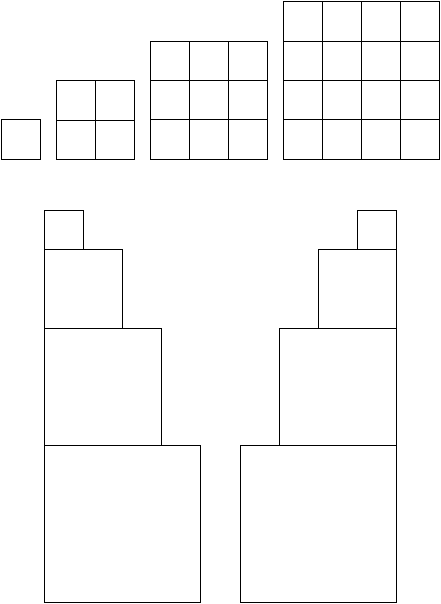
\includegraphics[scale=0.4]{FiguresMaths/SumSquares1}
\caption{Computing the sum of squares: initial configuration.}
       \label{fig:sumSquares1}
\end{center}
\end{figure}
\begin{figure}[ht]
\begin{center}
       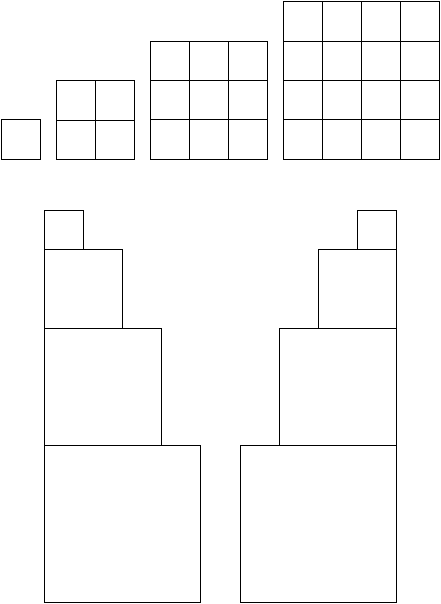
\includegraphics[scale=0.4]{FiguresMaths/SumSquares2}
\caption{Step 1 for computing the sum of squares: fill in the surface at the bottom.}
       \label{fig:sumSquares2}
\end{center}
\end{figure}
\begin{figure}[ht]
\begin{center}
       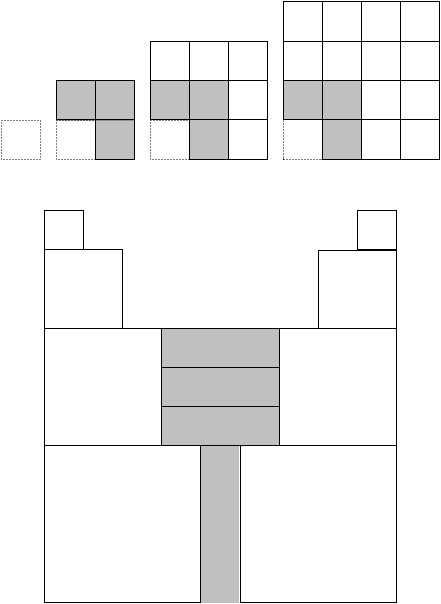
\includegraphics[scale=0.4]{FiguresMaths/SumSquares3}
\caption{Step 2 for computing the sum of squares.}
       \label{fig:sumSquares3}
\end{center}
\end{figure}
\begin{figure}[ht]
\begin{center}
       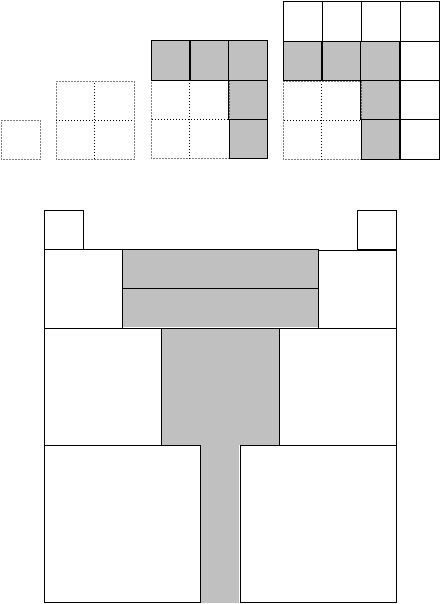
\includegraphics[scale=0.4]{FiguresMaths/SumSquares4}
\caption{Step 3 for computing the sum of squares.}
       \label{fig:sumSquares4}
\end{center}
\end{figure}
\begin{figure}[ht]
\begin{center}
       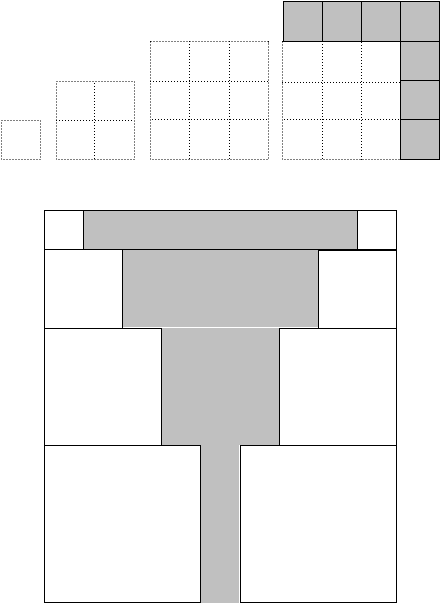
\includegraphics[scale=0.4]{FiguresMaths/SumSquares5}
\caption{Final step for computing the sum of squares: the rectangle is filled.}
       \label{fig:sumSquares5}
\end{center}
\end{figure}
**********************}

We begin to illustrate the technique of bounding summations via
integrals by focusing on summations of the form
\[ S_c(n) \ \eqdef \ \sum_{i=1}^n \ i^c, \]
for arbitrary positive numbers $c$.  The reader can garner intuition
for the upcoming bounds from the general shape of the rectangles and
continuous curves in Figs.~\ref{fig:riemann-n2-1}
and~\ref{fig:riemann-n2-2} We obtain our upper bound on $S_c(n)$ by
evaluating the integral that yields the area $\overline{C}_c(n)$ under
the lefthand continuous curve ($a$) in Fig.~\ref{fig:riemann-n2-1},
namely,
\begin{eqnarray}
\label{eq:upper-integral-xc}
\overline{C}_c(n) \ = \
\int_0^n \ (x+1)^c dx & = &
%  \int_0^n \ x^2 dx \ + \ 2 \int_0^n \ x dx \ + \ \int_0^n \ dx \\
% & = & \frac{1}{3} n^3 \ + n^2 \ + \ n \ + \ O(1).
 \frac{1}{c+1} (n+1)^{c+1} \ + \ O(1) \\
\nonumber
 & = & \frac{1}{c+1} n^{c+1} \ + \ O(n^c).
\end{eqnarray}
We obtain our lower bound on $S_c(n)$ by evaluating the integral that
yields the area $\underline{C}_c(n)$ under the righthand continuous
curve ($b$) in Fig.~\ref{fig:riemann-n2-2}, namely,
\begin{equation}
\label{eq:lower-integral-xc}
\underline{C}_c(n) \ = \
\int_1^n \ x^c dx \ = \ \frac{1}{c+1} n^{c+1} \ + \ O(1).
\end{equation}
Combining these bounds, we finally have the following two-sided bound
on $S_c(n)$.
\begin{equation}
\label{eq:bounds-sum-xc}
\frac{1}{c+1} n^{c+1} \ + \ O(1)
  \ \ \leq \ \ S_c(n)
  \ \ \leq \ \ \frac{1}{c+1} n^{c+1} \ + \ O(n^c).
\end{equation}
The main message here is:
\begin{center}
{\em The behavior of $S_c(n)$ as a function of $n$ is dominated by
  $\displaystyle \frac{1}{c+1} n^{c+1}$ as $n$ grows without bound.  }
\end{center}


\subsubsection{Nonnegative integer $c$th powers}
\label{sec:positive-integer-power}

\paragraph{\sf A. A better bound via the Binomial Theorem}
When $c$ is a positive integer, the following special case of Newton's
{\it Binomial Theorem}.\footnote{The general form of the Binomial
  Theorem expands the polynomial $(x+y)^k$ rather than $(x+1)^k$.  See
Section~\ref{sec:Binomial-thm}.}
\index{The Binomial Theorem!restricted form}
affords us a much more detailed version of the upper bound
(\ref{eq:upper-integral-xc})
%(\ref{eq:bounds-sum-xc})
on the sum $S_c(n)$.

\begin{theorem}[The Restricted Binomial Theorem]
\label{thm:restricted-binomial-thm}
For all positive integers $k$,\footnote{See (\ref{eq:binom-coeff}) for
  the definition of, and notation for, the binomial coefficient
  $\displaystyle {k \choose i}$.}
\[ (x+1)^k \ = \
\sum_{i=0}^k \ \ {k \choose i} x^{k-i}.
\]
\end{theorem}

We obtain our improved upper bound on $S_c(n)$ by parallelling the
reasoning that led us to the relation (\ref{eq:upper-integral-xc}).
Our improved upper bound emerges also by evaluating the integral that
yields the area $\overline{C}_c(n)$ under the continuous curve that
passes through the upper lefthand corners of the unit-width rectangles
specified by summation $S_c(n)$.
\begin{eqnarray}
\label{eq:upper-integral-xk}
\overline{C}_c(n) \ = \
\int_0^n \ (x+1)^c dx & = &
\int_0^n \ \left(\sum_{i=0}^c \ \ {c \choose i} x^{c-i} \right) dx \\
\nonumber
& = &
\sum_{i=0}^c \left( \int_0^n \  {c \choose i} x^{c-i} \right) dx \\
\nonumber
  & = &
\sum_{i=0}^c \ \ \frac{1}{c-i+1} {c \choose i} n^{c-i+1} \ + \ O(1)
\end{eqnarray}
This is a proper upper bound because the region defined by this curve
totally contains the region subtended by the rectangles.

\noindent
Using this strategy, we find that for any positive integer $c$,
summation $S_c(n)$ enjoys the following two-sided bound:
\begin{equation}
\label{eq:bounds-sum-xk}
\frac{1}{c+1} n^{c+1} \ + \ O(1)
  \ \ \leq \ \ \sum_{i=1}^n \ i^c
  \ \ \leq \ \ 
\sum_{i=0}^c \ \ \frac{1}{c-i+1} {c \choose i} n^{c-i+1} \ + \ O(1)
\end{equation}

We have, of course, not changed the dominant behavior of $S_c(n)$ as
$n$ grows without bound, but we have taken a substantial step toward
developing explicit expressions for the summations $S_c(n)$ when $c$
is a positive integer.

\medskip

\paragraph{\sf B. Using {\em undetermined coefficients} to refine sums}
We now introduce the {\em Method of Undetermined Coefficients}
\index{Method of Undetermined Coefficients}
and illustrate how to use it to derive explicit expressions for the
sums $S_c(n)$ when $c$ is a positive integer.  Our development builds
on the intuition garnered from the bounds (\ref{eq:bounds-sum-xk})
that
\[ S_c(n) \ = \ \frac{1}{c+1} n^{c+1} \ + \ a^{(c)}_c n^c \ + \
a^{(c)}_{c-1} n^{c-1} \ + \ \cdots \ + \ a^{(c)}_2 n^2 \ + \ a^{(c)}_1 n
 + \ a^{(c)}_0
\]
for some nonnegative numbers  
%$a^{(c)}_{c+1}$, 
$a^{(c)}_c$, \ldots,
$a^{(c)}_0$.  To begin, we know that $a^{(c)}_0 = 0$, because $S_c(0)
= 0$.
\begin{quote}
{\em Because we are beginning with a conjecture based on intuition, we
  will have to verify the explicit expressions that we derive.  We do
  this after deriving our expressions.}
\end{quote}

Because the Method becomes computationally cumbersome for large values
of $c$, we introduce the reader to it via the first few integer values
of $c$.

{\it The case $c=1$.}
%
We begin with the sum $S_1(n)$, whose value we already know.
Reasoning from the case $c=1$ of (\ref{eq:bounds-sum-xk}), we intuit
that
\[ S_1(n) \ = \ \frac{1}{2} n^2 \ + \ a^{(1)}_1 n \]
for some positive {\it undetermined coefficient} $a^{(1)}_1$.  We can
discover the value of the single unknown, $a^{(1)}_1$ by evaluating
$S_1(n)$ at any single value for the variable $n$.  Any value of $n$
will work; using the {\em smallest} one, $n=1$, simplifies our
calculation.

Because $S_1(1) = 1$, we have
\[ S_1(1) \ = \ 1 \ = \ \frac{1}{2} \ + \ a^{(1)}_1. \]
Therefore, $a^{(1)}_1 = 1/2$, which gives us yet one more derivation
of the value
\[ S_1(n) \ = \ \frac{1}{2} \left( n^2 + n \right) \ = \ 
\frac{n(n+1)}{2}.
\]

\medskip

{\it The case $c=2$.}
%
We derive an explicit expression for $S_2(n) \ \eqdef \  1 + 4 +
\cdots + n^2$.

\begin{prop}
{\em For all} $n \in \N$,
\begin{equation}
\label{eq:sum-1-to-nsq}
S_2(n) \ \eqdef \ \sum_{i=1}^n \ i^2 
 \ = \ \frac{1}{3} n^3 \ + \ \frac{1}{2} n^2 \ + \ \frac{1}{6} n
\end{equation}
\end{prop}

\noindent
$S_2(n)$ is often expressed in a more aesthetic form:
\[ S_2(n) \ = \
\frac{1}{6} n (n+1)(2n+1) \ = \
\frac{2n+1}{3} \cdot {n \choose 2}.
\]

\begin{proof}
Reasoning from the case $c=2$ of (\ref{eq:bounds-sum-xk}), we
propose the conjecture that
\begin{equation}
\label{eq:symbolic-cubic}
S_2(n) \ \ = \ \
\sum_{i=0}^n \ i^2 \ \ = \ \ \frac{1}{3} n^3 + a^{(2)}_2 n^2 + a^{(2)}_1 n.
\end{equation}
for some positive {\it undetermined coefficients} $a^{(2)}_2$ and
$a^{(2)}_1$.  We thereby express $S_2(n)$ as a polynomial in two
unknowns, $a^{(2)}_2$ and $a^{(2)}_1$.  We can determine values for
the unknowns by instantiating the polynomial with (any) two values of
$n$; to simplify calculations, we select the smallest two values of
$n$, namely, $n = 1,2$.  These instantiations of the polynomial leave
us with the following pair of linear equations.
\[
\begin{array}{cccccl}
n=1: & \sum_{i=0}^1 \ i^2
   & = & 1 & = &
1/3 \ + \ a^{(2)}_2 \ + \ a^{(2)}_1 \\
 & & & & & \\
n=2: & \sum_{i=0}^2 \ i^2
   & = & 5 & = &
8/3 \ + \ 4 a^{(2)}_2 \ + \ 2 a^{(2)}_1
\end{array}
\]
By elementary arithmetic, these equations simplify to yield the pair
\[
\begin{array}{ccc}
a^{(2)}_2 \ + \ a^{(2)}_1   & = & 2/3 \\
 & & \\
2 a^{(2)}_2 \ + \ a^{(2)}_1 & = & 7/6
\end{array}
\]
These equations reveal that
\[ 2/3 \ - \ a^{(2)}_2 \ = \ 7/6 \ - \ 2 a^{(2)}_2 \]
so that 
\[ a^{(2)}_2 \ = \ 1/2 \]
which means that
\[ a^{(2)}_1 \ = \ 1/6. \]
We have, thus, derived equation~(\ref{eq:sum-1-to-nsq}).  
\end{proof}

\medskip

We verify our expressions for $S_1(n)$ and $S_2(n)$ by induction in
subsection C.

\medskip

With more (calculational) work, but no new (mathematical) ideas, one
can derive explicit expressions for the sum of the first $n$ $c$th
powers, i.e., the sum $S_c(n)$, for any positive integer $c$.


\medskip

\paragraph{\sf C. Validating approximate summations via induction}
We employ the proof technique of (Finite) Induction by proving the
correctness of three summation formulas that have occupied our
attention in this chapter:
\begin{enumerate}
\item
the sum $S_1(n)$ of the first $n$ positive integers; cf., equation
(\ref{eq:sum-1-to-n})

\item
the sum $S_2(n)$ of the squares of the first $n$ positive integers;
cf., equation (\ref{eq:sum-1-to-nsq})

\item
the sum of the first $n$ odd positive integers; cf.,
Proposition~\ref{thm:squares-odd-integers-Gauss}.
\end{enumerate}
We deal with these formulas in turn.

\noindent {\it 1. Verifying equation (\ref{eq:sum-1-to-n}) for $S_1(n)$.}
%
For every positive integer $m$, let {\bf P}$_1(m)$ be the proposition
\[  1 \ + \ 2 \ +  \cdots  + \ m \ = \ {{m+1} \choose 2}. \]
We proceed according to the standard format of an inductive argument.

\begin{description}
\item[{\sf The base case P$_1(1)$}.]
%
Because ${\displaystyle {2 \choose 2}} = 1$, proposition {\bf P}$_1(1)$
is true.

\item[{\sf The inductive hypothesis}.]
%
Assume, for the sake of induction, that proposition {\bf P}$_1(m)$ is
true for every positive integer $m < n$.  In particular, then,
proposition {\bf P}$_1(n-1)$ is true.

\item[{\sf Extending the induction}.]
%
Because proposition {\bf P}$_1(n-1)$ is true, we know that
\[ S_1(n-1) \ = \ 1 + 2 + \cdots + (n-1) \ = \ {n \choose 2}.  \]
By direct calculation, then,
\begin{eqnarray*}
S_1(n) & = & {n \choose 2} + n \\
  & = & \frac{n(n-1)}{2}  \ + \ n \\ 
%  & = & \frac{n^2 - n + 2n}{2} \\
  & = & \frac{n^2 + n}{2} \\
  & = & {{n+1} \choose 2},
\end{eqnarray*}
as was verified in equation (\ref{eq:sum-1-to-n}).
\end{description}
Because $n$ is an arbitrary positive integer, we conclude that
{\bf P}$_1(n)$ is true whenever
\begin{itemize}
\item
{\bf P}$_1(1)$ is true
\item
{\em and}
{\bf P}$_1(m)$ is true for all $m < n$.
\end{itemize}
By the Principle of (Finite) Induction, then, we conclude that
proposition {\bf P}$_1(n)$ is true for all positive integers $n$.
\qed

\bigskip


\noindent {\it 2. Verifying equation (\ref{eq:sum-1-to-nsq}) for $S_2(n)$.}
%
For every positive integer $m$, let {\bf P}$_2(m)$ be the proposition
\[  1 \ + \ 2^2 \ + \ 3^2 \ + \cdots + \ m^2 \ = \ 
\frac{1}{6} m (m+1)(2m+1).
\]
We proceed according to the standard format of an inductive argument.

\begin{description}
\item[{\sf The base case P$_2(1)$}.]
%
Because ${\displaystyle \frac{1}{6} (2 \cdot 3)} = 1$, proposition {\bf
    P}$_2(1)$ is true.

\item[{\sf The inductive hypothesis}.]
%
Assume, for the sake of induction, that proposition {\bf P}$_2(m)$ is
true for every positive integer $m < n$.  In particular, then,
proposition {\bf P}$_2(n-1)$ is true.

\item[{\sf Extending the induction}.]
%
Because proposition {\bf P}$_2(n-1)$ is true, we know that
\[ S_2(n-1) \ = \
\frac{1}{6} (n-1) \cdot n \cdot (2n-1).
\]
By direct calculation, then,
\begin{eqnarray*}
S_2(n) & = &
\frac{1}{6} (n-1) \cdot n \cdot (2n-1) \ + \ n^2 \\
  & = &
\frac{n}{6} \left( (n-1) \cdot (2n-1) + 6n \right) \\
  & = & \frac{n}{6} \left( 2n^2 +3n + 1 \right) \\ 
  & = & \frac{n}{6} (n+1)(2n+1),
\end{eqnarray*}
as was verified in equation (\ref{eq:sum-1-to-nsq}).
\end{description}
Because $n$ is an arbitrary positive integer, we conclude that
{\bf P}$_2(n)$ is true whenever
\begin{itemize}
\item
{\bf P}$_2(1)$ is true
\item
{\em and}
{\bf P}$_2(m)$ is true for all $m < n$.
\end{itemize}
By the Principle of (Finite) Induction, then, we conclude that
proposition {\bf P}$_2(n)$ is true for all positive integers $n$.
\qed


\bigskip

\noindent {\it 3. Verifying that each perfect square $n^2$ is
  the sum of the first $n$ odd integers.}
%
We turn finally to the assertion that, for every positive integer $n$,
\[ n^2 \ = \ 1 \ + \  3 \ + \ 5 \ + \cdots + \ 2n-1. \]
For each positive integer $n$, let {\bf P}$(n)$ denote the proposition
that the preceding equation holds.

The following inductive proof complements the constructive proofs of
the same result in Proposition~\ref{thm:squares-odd-integers-Gauss}.
We proceed according to the standard format of an inductive argument.

\begin{description}
\item[{\sf The base case P$(1)$}.]
%
Because $1$ is a perfect square, proposition {\bf P}$(1)$ is true.

\item[{\sf The inductive hypothesis}.]
%
Assume, for the sake of induction, that proposition {\bf P}$(m)$ is
true for every positive integer $m < n$.  In particular, then,
proposition {\bf P}$(n-1)$ is true.

\item[{\sf Extending the induction}.]
%
Because proposition {\bf P}$(n-1)$ is true, we know that
\[ 
 1 + 3 + 5 + \cdots + 2n-3 + 2n-1 \ = \ (n-1)^2 + 2n-1.  \]
By direct calculation, we see that
\[ (n-1)^2 + 2n-1 \ = \ (n^2 -2n +1) + (2n-1) \ = \ n^2. \]
\end{description}
Because $n$ is an arbitrary positive integer, we conclude that
{\bf P}$(n)$ is true whenever
\begin{itemize}
\item
{\bf P}$(1)$ is true
\item
{\em and}
{\bf P}$(m)$ is true for all $m < n$.
\end{itemize}
By the Principle of (Finite) Induction, then, we conclude that {\bf
  P}$(n)$ is true for all $n \in \N^+$.
\qed


\subsubsection{$S_c(n)$ for general {\em negative} $c$th powers}
\label{sec:sum-of-i2c<0}

We focus finally on summations of the form
\[ S_c(n) \ \eqdef \ \sum_{i=1}^n \ i^c, \]
for arbitrary {\em negative} numbers $c$.  The reader can garner
intuition for the upcoming bounds from the general shape of the
rectangles and continuous curves in Figs.~\ref{fig:riemann-harmonic1}
and~\ref{fig:riemann-harmonic2}.

\begin{prop}
\label{thm:general-bounds-negative-xc}
For summations $S_c(n)$ with fixed negative powers $c<0$,
\begin{equation} 
\label{eq:general-bounds-negative-xc}
\left[
\underline{C}_c(n) \ = \
\int_0^{n-1} \ (x+1)^c dx
\right]
\ \leq \ S_c(n) \ \leq \
\left[
\overline{C}_c(n) \ = \
\int_1^n \ x^c dx
\right].
\end{equation}
\end{prop}

\begin{proof}
We obtain our upper bound on the sum of $S_c(n)$ by evaluating the
integral that yields the area $\overline{C}_c(n)$ under the righthand
continuous curve ($a$) in the analogue of
Fig.~\ref{fig:riemann-harmonic1} for $S_c(n)$.  We obtain our lower
bound on $S_c(n)$ by evaluating the integral that yields the area
$\underline{C}_c(n)$ under the lefthand continuous curve ($b$) in the
analogue of Fig.~\ref{fig:riemann-harmonic2} for $S_c(n)$.
\end{proof}

When $c \neq -1$,\footnote{We need to avoid the case $c = -1$ so that
  we do not attempt to divide by $0$.}~we can provide more detail,
using reasoning similar to that underlying the bounds
(\ref{eq:bounds-sum-xc}) that hold for positive values of $c$.

\paragraph{\sf A. Negative powers $c$ with $-1 < c < 0$}
In this case, we obtain essentially the same bounds as in the case of
nonnegative $c$.  To wit,

\begin{prop}
\label{thm:bounds-(-1)<c<0}
For sums $S_c(n)$ with fixed negative powers in the range $-1 < c<0$,
\begin{equation}
\label{eq:bounds-(-1)<c<0}
\begin{array}{l}
\mbox{For $-1 < c< 0$:} \\
 \\
\hspace*{.35in}
{\displaystyle \frac{1}{c+1} n^{c+1} \ - \ O(n^c)}
  \ \ \leq \ \ S_c(n)
  \ \ \leq \ \
{\displaystyle \frac{1}{c+1} n^{c+1} \ + \ O(1)}.
\end{array}
\end{equation}
The infinite version of summation $S_c(n)$, namely, the series
\[ S_c^{(\infty)} \ \eqdef \ \sum_{i=0}^\infty i^c \]
diverges.
\end{prop}

We thus observe that $S_c(n)$ has the same growth {\em pattern} as $n$
grows as it does when $c$ is positive, but that $S_c(n)$'s growth {\em
  rate} is slower because of the damping effect the negative $c$ in
the exponent.  This damped growth notwithstanding, the infinite series
$S_c^{(\infty)}$ diverges because $n^{c+1}$, which is the variable
portion of the lower bound on $S_c(n)$, grows without bound as $n$
grows without bound.

\paragraph{\sf B. Negative powers $c$ with $c < -1$}
When $c$ is ``very negative'', specifically, when $c < -1$, then the
infinite version of $S_c(n)$, call it $S_c^{(\infty)}$, is a {\em
  convergent} infinite series.  Because $n^c$ {\em shrinks} in this
case as $n$ grows, an analysis mirroring the one that leads to
(\ref{eq:bounds-(-1)<c<0}) provides the following sum for $S_c^{(\infty)}$.

\begin{prop}
\label{thm:bounds-negative-(not-1)-sum-xc}
When the fixed negative power $c$ is smaller than $-1$, then the
infinite version, $S_c^{(\infty)}$, of $S_c(n)$, converges, with the
following sum.
\begin{equation}
\label{eq:bounds-negative-(not-1)-sum-xc}
S_c^{(\infty)} \ = \ \frac{1}{c+1}
\end{equation}
\end{prop}

\begin{proof}
We see as in (\ref{eq:bounds-(-1)<c<0}) that, for $c<-1$, as $n$ grows
without bound, $S_c(n)$ tends to the value ${\displaystyle
  \frac{1}{c+1}}$.
\end{proof}

\paragraph{\sf C. Negative powers $c$ with $c = -1$: the {\em harmonic} summation}
The singular case defined by the value $c = -1$ defines the important
{\it harmonic series},
\index{harmonic series $S^{(H)}$}
\[ S^{(H)} \ = \ \sum_{i=1}^\infty \ \frac{1}{i} \]
and its finite prefixes that comprise the {\it harmonic summation}
\[ S^{(H)}(n) \ = \ \sum_{i=1}^n \ \frac{1}{i} \]
\index{harmonic summation $S^{(H)}(n)$}


{\it (i) The asymptotic behavior of $S^{(H)}(n)$.}
\index{harmonic summation $S^{(H)}(n)$!asymptotic behavior}
%
It has been known since the time of the well-traveled Swiss
mathematician Leonhard Euler \index{Euler, Leonhard} that $S^{(H)}$
and $S^{(H)}(n)$ are closely related to the {\em natural}, or,
\index{Napier, John}
{\it Napierian},\footnote{The natural logarithm, i.e., the logarithm
  to the base $e$, is commonly referred to as the {\it Napierian
    logarithm}, in honor of the Scottish polymath John
  Napier.}~logarithm $\ln n$, \textit{i.e.}, the logarithm whose base is
Euler's constant \index{Euler's constant} $e = 2.718281828 \ldots$.

\begin{prop}
\label{thm:harmonic}
The behavior of the harmonic summation $S^{(H)}(n)$ as a function of
$n$ is given by
\[ S^{(H)}(n) \ \approx \ \ln n. \]
It follows, in particular, that the harmonic series $S^{(H)}$ diverges.
\end{prop}

\begin{quote}
\index{harmonic series  $S^{(H)}$!relation to music}
{\em The adjective ``harmonic'' calls to mind a number of concepts
  associated with {\em music}, such as ``harmonics'' and ``harmony''.
  The association between our series and these musical concepts is not
  a coincidence.  The name of the harmonic series derives from the
  concept of {\em overtones}, or {\em harmonics}, in music.  When one
  observes a vibrating string, one finds that the wavelengths of its
  overtones, as fractions of the string's fundamental wavelength, are
  the terms of the {\em harmonic sequence}, namely, $\frac{1}{2}$,
  $\frac{1}{3}$, $\frac{1}{4}$, \ldots.  }
\end{quote}

%{\Denis I developed a graphical way to interpret the harmonic sum and its link with the neperian log (this is I believe very interesting and original.
%May be this is the wrong place, tell me (we can also split the
%following into smaller pieces...)}

{\it (ii) Bounds on the asymptotic behavior of $S^{(H)}(n)$.}
\index{harmonic summation $S^{(H)}(n)$!understanding logarithmic behavior}
%
Fig~\ref{fig:HarmonicSumInitial} depicts the harmonic summation
$S^{(H)}(n)$ as the area of abutting unit-width rectangles of
respective heights (from left to right) of $1$, $1/2$, $1/3$, \ldots,
$1/n$.
\begin{figure}[htb]
\centerline{
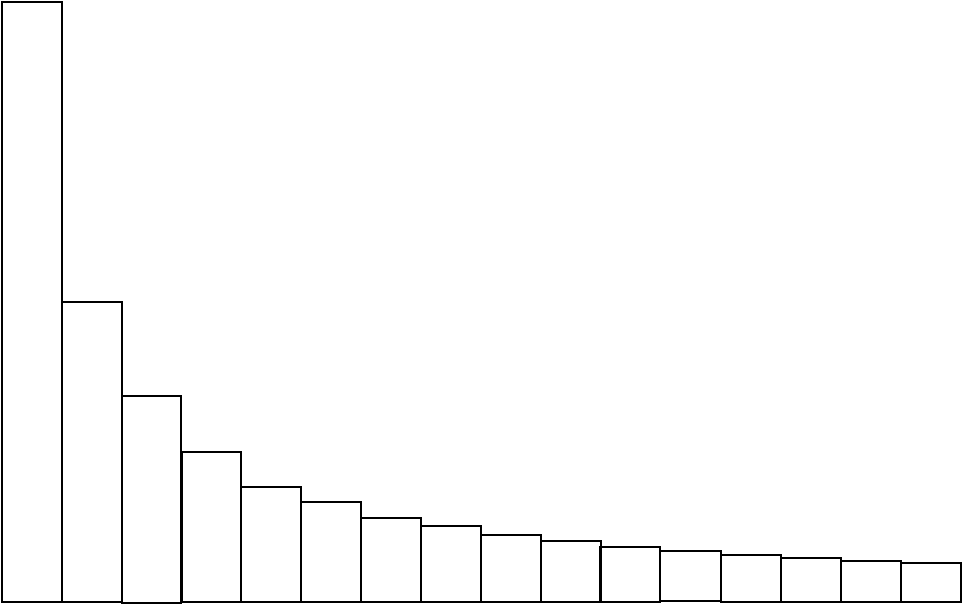
\includegraphics[scale=0.3]{FiguresMaths/HarmonicSumInitial}
}
\caption{The harmonic summation $S^{(H)}(n)$ represented by the area
  of abutting unit-width rectangles of decreasing heights.}
\label{fig:HarmonicSumInitial}
\end{figure}

In order to better understand the behavior of $S^{(H)}(n)$ as a
function of $n$, let us group the summation's consecutive terms into
subsums composed from groups of summands whose sizes are consecutive
powers of $2$:
\begin{eqnarray*}
\left( 1 \right) \ + \ \left( \frac{1}{2} + \frac{1}{3} \right)
 & + & \left( \frac{1}{4} + \frac{1}{5} + \frac{1}{6} + \frac{1}{7} \right) \\
 & + & \left( \frac{1}{8} +\frac{1}{9} + \frac{1}{10} + \frac{1}{11}
       + \frac{1}{12} + \frac{1}{13} + \frac{1}{14} + \frac{1}{15} \right) \ + \cdots
\end{eqnarray*}
Next, we isolate each grouped subsum and list the subsums in order of
size, measured as number of inverse-integer summands.
\[ \begin{array}{llcl}
\mbox{Sum of $(2^0 =1)$ consecutive inverses:} &
A_0 & = &  {\displaystyle 1 } \\
\mbox{Sum of $(2^1 =2)$ consecutive inverses:} &
A_1 & = &  {\displaystyle \frac{1}{2} + \frac{1}{3} }  \\
\mbox{Sum of $(2^2 =4)$ consecutive inverses:} &
A_2 & = &  {\displaystyle \frac{1}{4} + \frac{1}{5} + \frac{1}{6} + \frac{1}{7} } \\
 & \vdots & & \vdots \\
\mbox{Sum of $2^i$ consecutive inverses:} &
A_i & = &  {\displaystyle \frac{1}{2^i} + \frac{1}{2^i+1} + \cdots +
     \frac{1}{2^{i+1}-1}  } \\
 & \vdots & & \vdots \\
\end{array}
\]

Finally, we derive absolute-constant upper and lower bounds that hold
for all of the subsums.  To derive these bounds, we focus on the
generic subsum $A_i$, which consists of $2^i$ summands.  When we focus
on the largest and smallest inverse-integers in $A_i$---which are,
respectively, $1/2^i$ and $1/(2^{i+1}-1)$---we note the following
absolute bounds.
\[
\frac{1}{2}
 \ < \
\frac{2^i}{2^{i+1}-1}
 \ < \
2^i \cdot A_i
  \ < \
\frac{2^i}{2^i}
  \ = \ 1
\]
We thereby have absolute constant upper and lower bounds on every 
subsum $A_i$.

Referring back to Fig.~\ref{fig:HarmonicSumInitial}, what the
just-derived bounds mean is the following.  Let us proceed left to
right along the abutting rectangles in the figure, and let us recall,
from Section~\ref{sec:exponential+logarithm}.B, the definition of
``logarithm to the base $b$''.  As we double the number of rectangles
we have traversed:
\begin{enumerate}
\item
We increase the aggregate area of the thus-far traversed rectangles by
at most $1$.

{\em This means that $S^{(H)}(n)$ grows no faster than $\log_2 n$.}

\item
We increase the aggregate area of the thus-far traversed rectangles by
more than $1/2$.

{\em This means that $S^{(H)}(n)$ grows faster than $\log_4 n$.}
\end{enumerate}
Of course, these observations are consistent with the verified actual
natural-logarithmic growth rate of $S^{(H)}(n)$, because $2 < e < 4$.

\begin{figure}[htb]
\centerline{
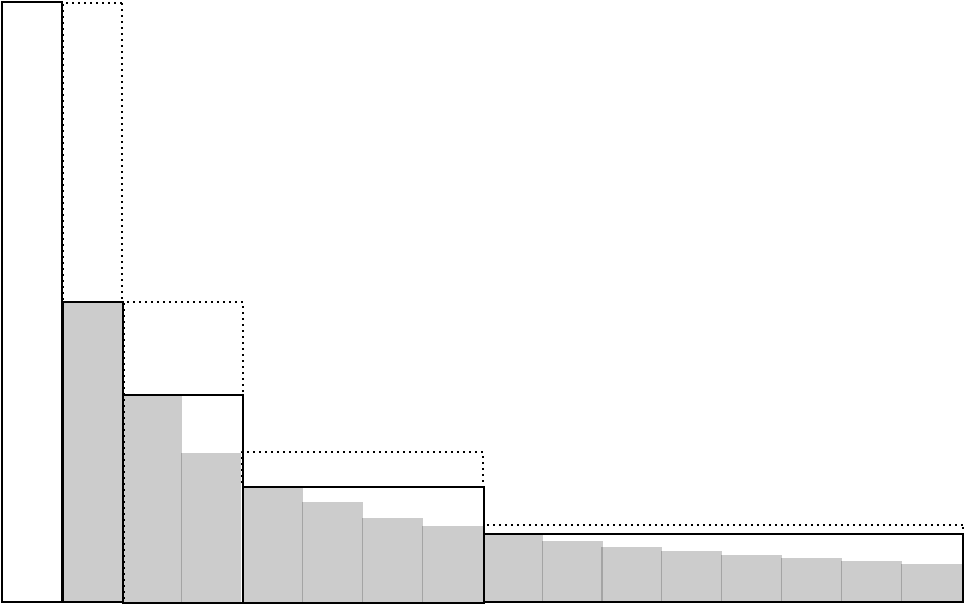
\includegraphics[scale=0.3]{FiguresMaths/HarmonicSumUpperbound}
}
\caption{Upper bound of $A_i$ by larger unit-size rectangles in the harmonic sum.}
\label{fig:HarmonicSumUpperbound}
\end{figure}

\begin{figure}[htb]
\centerline{
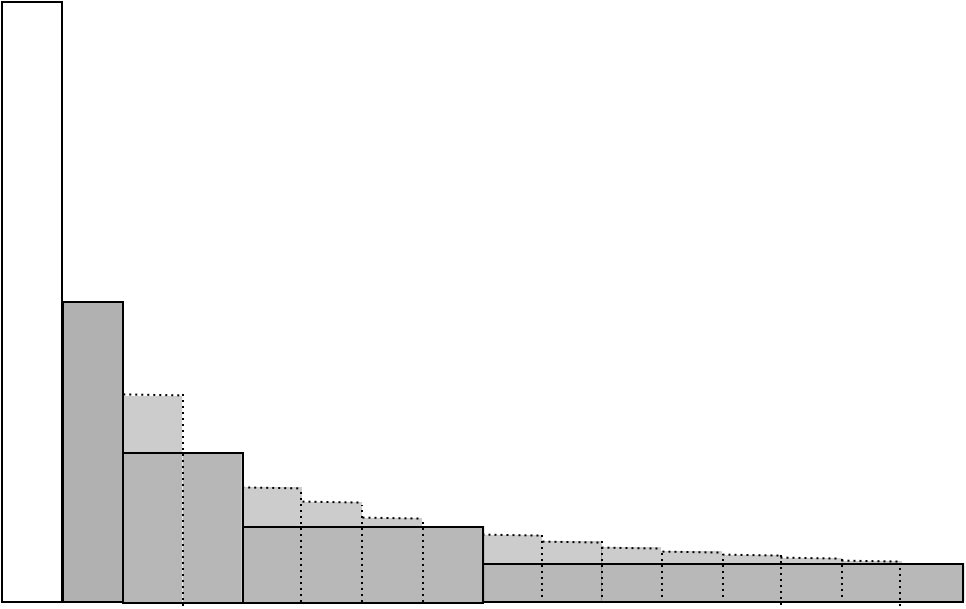
\includegraphics[scale=0.3]{FiguresMaths/HarmonicSumLowerbound}
}
\caption{A pictorial lower bound for the harmonic summation.}
\label{fig:HarmonicSumLowerbound}
\end{figure}



\ignore{**************
%and more generally, $A_i$ is the sum of the consecutive $\frac{1}{i}$
%(for $k$ such that $\frac{1}{2^i+1} \leq k \leq \frac{1}{2^{i+1}}$). 
Note that each $A_i$ is the sum of $2^i$ consecutive terms.

We claim that each partial sum satisfies $A_i \leq 1$.  Verifying this
by actually summing each $A_i$ requires a bit of calculation, but if
we want only the bound, then we achieve that quite easily from the
drawing in Fig~\ref{fig:HarmonicSumUpperbound}.
\begin{figure}[htb]
\centerline{
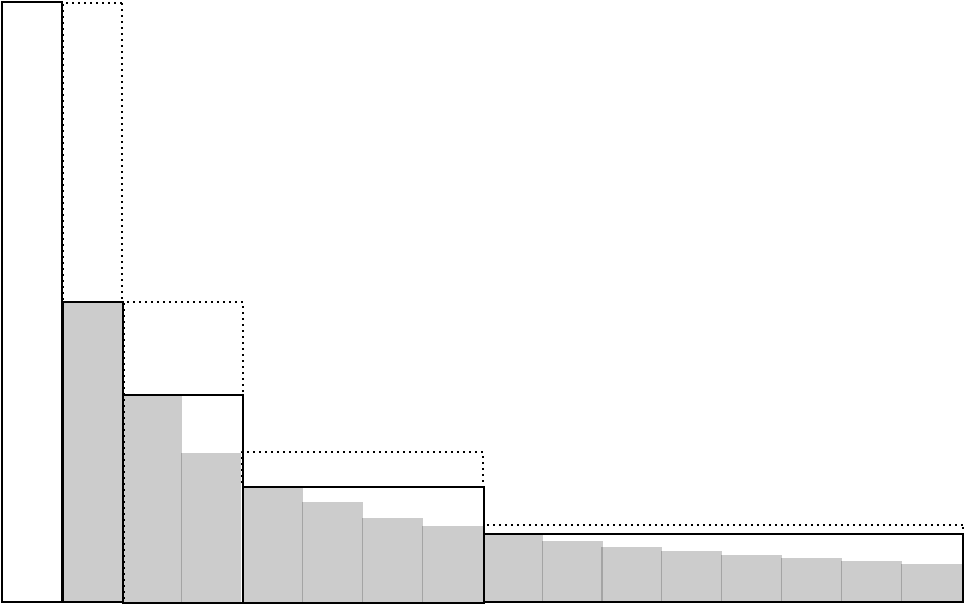
\includegraphics[scale=0.3]{FiguresMaths/HarmonicSumUpperbound}
}
\caption{Upper bound of $A_i$ by larger unit-size rectangles in the harmonic sum.}
\label{fig:HarmonicSumUpperbound}
\end{figure}

constant value $k$.  This claim is verified with the value $k=1$ by
the drawing in Fig~\ref{fig:HarmonicSumUpperbound}. shows that all the
$A_i$ are lower than $1$ but we could have considered a more accurate
value, however, it is enough and simple.  This result is obtained by
embedding each term $A_i$ by larger rectangles (of unit surfaces), the
upper bound is the bold rectangle plus the dashed rectangle at the
top.  {\Denis I hope my previous explanation is clear enough...}


Going into more detail, we claim that the partial sums $A_i$ form an
increasing sequence.  Here again, an exact verification by calculating
each $A_i$ is onerous to achieve, but the claim can be verified
graphically from the drawing in Fig~\ref{fig:HarmonicSumLowerbound}.
\begin{figure}[htb]
\centerline{
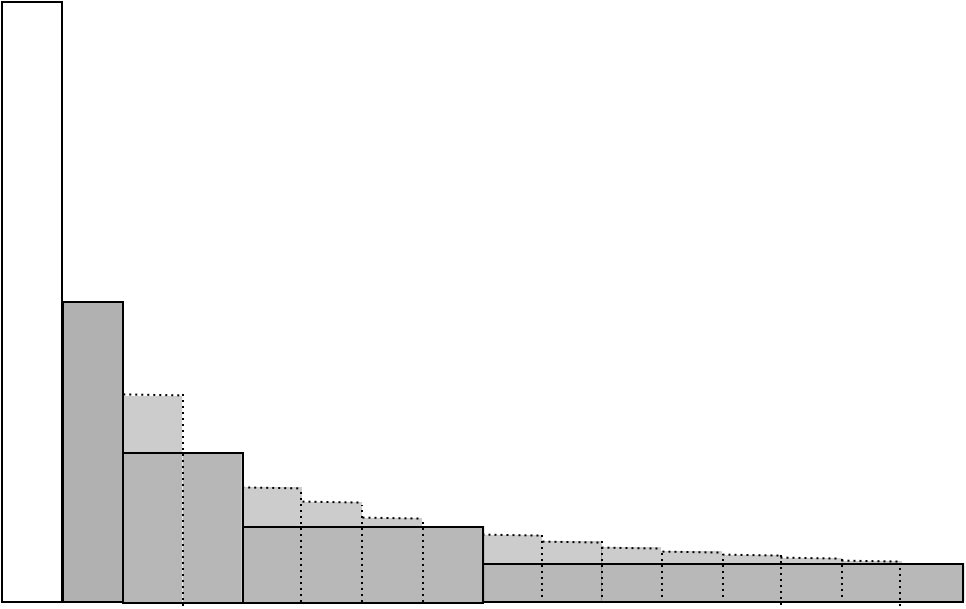
\includegraphics[scale=0.3]{FiguresMaths/HarmonicSumLowerbound}
}
\caption{A pictorial lower bound for the harmonic summation.}
\label{fig:HarmonicSumLowerbound}
\end{figure}
The drawing suggests the following exact sequence of analyses.

Let us verify first that $A_2 \geq A_1$ by showing that $A_2-A_1 \geq
0$; this inequality corresponds to the leftmost light grey rectangle
in Fig~\ref{fig:HarmonicSumLowerbound}.  We want to sum
\[ A_2-A_1 \ = \ \frac{1}{5} + \frac{1}{6} + \frac{1}{7} + \frac{1}{8}
- \frac{1}{3} - \frac{1}{4} \]
Because $\displaystyle \frac{1}{5} \geq \frac{1}{6}$ and
$\displaystyle \frac{1}{7} \geq \frac{1}{8}$, we have
\[
A_2-A_1 \ \ \geq \ \
\left(\frac{1}{6} + \frac{1}{6}\right) - \frac{1}{3} +
\left(\frac{1}{8} + \frac{1}{8}\right) - \frac{1}{4}
  \ \ =  \ \  0.
\]
Hence, $A_2 \geq A_1$. 

We continue to use such grouped calculations to prove that each
$A_{i+1} \geq A_i$.  To wit, we group $\displaystyle \frac{1}{2^{i+1}
  + 1} + \frac{1}{2^{i+1} + 2}$ with $\displaystyle -\frac{1}{2^{i} +
  1}$.  Because $\displaystyle \frac{1}{2^{i+1} + 1} \geq
\frac{1}{2^{i+1} + 2}$, we have $\displaystyle \frac{1}{2^{i+1} + 1} +
\frac{1}{2^{i+1} + 2} - \frac{1}{2^{i} + 1} \geq 0$.  We conclude that
$A_{i+1} \geq A_i$.

Finally, as the sequence $A_i$ is bounded above and increasing, it converges to a constant.


The preceding grouping of the terms of $S^{(H)}(n)$, combined with our
bounds on the generic $A_i$


coupled with the
the fact that
The explanation relies on the following observations of the harmonic series:
$S^{H}(2^{i+1}-1) = S^{H}(2^{i}-1) + A_i$

From a given value of $i$, each $A_i$ and its successive values have roughly the same value equal to the limit of $A_i$.
In other words, we go from index $2^i$ to $2^{i+1}$ in $S^{H}$ by a multiplication by $2$ that corresponds to adding a constant. 
This is exactly what the log means!
***************}


